\documentclass[10pt]{amsart}

\usepackage{fullpage}
\usepackage{graphicx}
\usepackage{times}

\usepackage{amsmath}
\usepackage{url}
\usepackage{fancyvrb}
\usepackage{verbatim}
\usepackage{caption}
\usepackage{subcaption}
\usepackage{multirow}
\usepackage{floatrow}
\usepackage{proof-dashed}
\usepackage{amsthm}
\usepackage[numbers,sort]{natbib}
\usepackage[backref,pageanchor=true,plainpages=false, pdfpagelabels, bookmarks,bookmarksnumbered]{hyperref}
\usepackage{latexsym}
\usepackage{amssymb}            % for \multimap (-o)
\usepackage{stmaryrd}           % for \binampersand (&), \bindnasrepma (\paar)

\newcommand{\m}[1]{\mathsf{#1}}
\newcommand{\f}[1]{\framebox{#1}}

\newcommand{\eph}{\mathit{eph}}
\newcommand{\pers}{\mathit{pers}}
\newcommand{\um}[1]{\underline{\m{#1}}}

\newcommand{\seq}{\vdash}
\newcommand{\semi}{\mathrel{;}}
\newcommand{\lequiv}{\mathrel{\dashv\vdash}}

% symbols of linear logic
\newcommand{\lolli}{\multimap}
\newcommand{\tensor}{\otimes}
\newcommand{\with}{\mathbin{\binampersand}}
\newcommand{\paar}{\mathbin{\bindnasrepma}}
\newcommand{\one}{\mathbf{1}}
\newcommand{\zero}{\mathbf{0}}
\newcommand{\bang}{{!}}
\newcommand{\whynot}{{?}}
\newcommand{\bilolli}{\mathrel{\raisebox{1pt}{\ensuremath{\scriptstyle\circ}}{\lolli}}}
% \oplus, \top, \bot


\newcommand{\mz}{\m{match} \;}
\newcommand{\stepz}{\m{step} \;}
\newcommand{\tab}[0]{\;\;\;\;}
\newcommand{\dz}{\m{derive}~}
\newcommand{\comp}[0]{\m{comp} \;}
\newcommand{\az}{\m{apply} \;}
\newcommand{\doz}{\m{run} \;}
\newcommand{\seqnocut}[3]{#1 ; #2 \Rightarrow #3}
\newcommand{\defeq}{\buildrel\triangle\over =}
\newcommand{\compr}[1]{\m{def} \; #1}

\newcommand{\stepo}{\m{step}_{LLD} \;}
\newcommand{\mo}{\m{match}_{LLD} \;}
\newcommand{\contlld}{\m{cont}_{LLD}}
\newcommand{\cont}{\contlld \;}
\newcommand{\contclld}{\m{cont}_{LLDc}}
\newcommand{\contc}{\contclld \;}
\newcommand{\done}{\m{derive}_{LLD} \;}
\newcommand{\doo}{\m{run}_{LLD} \;}
\newcommand{\matchlldc}{\m{match}_{LLDc}}
\newcommand{\mc}[0]{\matchlldc \; }
\newcommand{\dall}[0]{\m{fix}_{LLD} \; }
\newcommand{\strans}[0]{\m{update}_{LLD} \;}
\newcommand{\dc}{\m{derive}_{LLDc} \;}
\newcommand{\ao}{\m{apply}_{LLD} \;}

\newcommand{\com}{\xrightarrow{*}}
%\mapsto}
\newcommand{\feq}[2]{#1 \equiv #2}

\begin{document}

\newcommand{\cmu}{\ensuremath{^\dag}}
\newcommand{\fcup}{\ensuremath{^\ddag}}

\title{Dynamic Semantics for a Concurrent Forward-Chaining Linear Logic Programming Language}
\author{Flavio Cruz\cmu\fcup, Frank Pfenning\cmu\\
       \cmu Carnegie Mellon University, Pittsburgh, PA 15213\\
       \url{{fmfernan, fp}@cs.cmu.edu} \\
       \fcup CRACS \& INESC TEC, Faculty of Sciences, University Of Porto\\
       Rua do Campo Alegre, 1021/1055, 4169-007 Porto, Portugal\\
       \url{flavioc@dcc.fc.up.pt}}

\newtheorem{lemma}{Lemma}[section]
\newtheorem{theorem}{Theorem}[section]
\newtheorem{definition}{Definition}[section]

\begin{abstract}
Thing
\end{abstract}

\maketitle

\section{Introduction}

Prolog~\cite{Colmerauer:1993:BP:154766.155362} is one of the first logic programming languages to become available, yet it still one the most popular logic programming language in use today. Prolog is a \emph{backwards-chaining} logic programming language where a program is composed of a set of rules that can be activated by inputing a query. Given a query $q(\hat{x})$, a Prolog interpreter will work backwards by matching $q(\hat{x})$ against the head of a rule. If found, the interpreter will then try to match the body of the rule, recursively, until it finds the program axioms (rules without body). If the search procedure succeeds, the interpreter finds a valid substitution for the $\hat{x}$ variables.

Datalog~\cite{Ramakrishnan93asurvey} is very popular logic programming language for deductive databases. Although it is a syntactic subset of Prolog, it works differently than Prolog because it is a \emph{forward-chaining} logic programming language. In Datalog, the program is composed of a database of facts $D$ and a set of rules $R$. Initially, the database $D$ starts with a set of axioms given by the program. Then, the interpreter will pick a subset of rules $R'$ of $R$ that can be applied using $D$. By applying $R'$, new facts are derived and added to the database.

Datalog interpreters usually employ a technique called \emph{Iterative Fixpoint Evaluation} (IFE) or \emph{semi-na\"{i}ve evaluation}~\cite{Ramakrishnan93asurvey} in order to generate the complete set of facts from the derivation rules. In IFE, computation is performed in iterations. In the first iteration, we consider all the axioms and
apply all rules that can be applied using the database. Once the database will be updated with the newly derived facts, we apply again all the rules given
the new database. If a rule is applied with at-least one fact that was derived in the previous iteration, then the facts instantiated by the head of the
rule can be added to the database. Otherwise, we ignore them since such facts must already been derived before. This is repeated until no new facts are
added to the database.

IFE takes advantage of the fact that Datalog is based on Horn clauses~\cite{journals/jsyml/Horn51} and is thus monotonic. When a rule is applied, new information is added to the database but not removed. The database can be implemented efficiently since facts are stored there until the program completes.

We have designed a new forward-chaining logic programming language called Linear Meld (LM). LM is similar to Datalog but uses linear logic~\cite{girard-87} as its foundation. Since linear logic is the \emph{logic of resources}, LM rules may consume facts from the database, which makes IFE impossible to use as
an evaluation strategy. LM is concurrent because the forward-chaining proof process is done at several places - called \emph{nodes} -
and derivation of facts may lead to communication between them. The communication paths between nodes and the nodes themselves create
a graph data structure where computation happens concurrently.
LM also includes novel features such as comprehensions and aggregates, which allow the programmer to iterate over
or accumulate values from the database, respectively.

In this paper, we want to present an high level dynamic semantics and then a low level dynamic semantics of LM.
Both semantics will be presented using proof-theoretic methods. The high level semantics will be very closely related to the linear logic sequent calculus.
The low level semantics will be much closer to a real implementation since it removes most of non-determinism of the high level semantics and
also describes in detail how the proof search mechanism works, including backtracking and resource management. We also relate both semantics by
proving that the low level dynamic semantics is sound in relation to the high level dynamic semantics.

The paper is organized as follows. In the first section, we give a brief overview of LM, including its syntax and how it works in practice.
Next, we present the connection between LM and linear logic, including the connectives used and how they relate to LM programs. We then present
the high level and low level dynamic semantics, followed by the soundness proof. Finally, we finish the paper with some conclusions.

\section{Related Work}
Linear logic has been used in the past as a basis for logic-based programming languages~\cite{Miller85anoverview}, including bottom-up and top-down programming languages. Lolli, a programming language presented in~\cite{Hodas94logicprogramming}, is based on a fragment of intuitionistic linear logic
and proves goals by lazily managing the context of linear resources during top-down proof search. LolliMon~\cite{Lopez:2005:MCL:1069774.1069778} is a concurrent linear logic programming language that integrates both bottom-up and top-down search, where bottom-up computations are encapsulated inside a monad and are concurrent, while top-down search is done sequentially. The programs starts by performing top-down search but this can be suspended in order to perform bottom-up search. This concurrent bottom-up search stops until a fix-point is achieved, after which top-down search is resumed. LolliMon is derived from the a concurrent logical framework called CLF~\cite{Watkins:2004uq,Cervesato02aconcurrent,Watkins03aconcurrent}.

As a bottom-up linear logic programming language, LM shares similarities with Constraint Handling Rules (CHR)~\cite{Betz:2005kx,Betz:2013:LBA:2422085.2422086}.
CHR is a concurrent committed-choice constraint language used to write constraint solvers. A CHR program is a set of rules and
a set of constraints (which can be seen as facts). Constraints can be consumed or generated during the application of rules.
Unlike LM, in CHR there is no
concept of rule priorities, but there is an extension to CHR that supports them~\cite{DeKoninck:2007:URP:1273920.1273924}.
Finally, there is also a CHR extension that adds persistent constraints and it has been proven to be sound and complete~\cite{DBLP:journals/corr/abs-1007-3829}.

\iffalse
Many programming languages . Although there are a few logic programming languages such as P2~\cite{Loo-condie-garofalakis-p2},
Meld~\cite{ashley-rollman-iclp09}, or Dedalus~\cite{Alvaro:EECS-2009-173} that already do this, they are based on classical logic, where facts are persistent. For most of these systems, there's no concept of state, except for Dedalus where state is modeled as time.

Graph Transformation Systems (GTS)~\cite{Ehrig:2004vn}, commonly used to model distributed systems, perform rewriting of graphs through
a set of graph productions. GTS also introduces
concepts of parallelism, where it may be possible to apply several transformations at the same time. In principle, it should be possible to model
LM programs as a graph transformation: we directly map the LM graph of nodes to GTS's initial graph and consider logical facts as nodes that are connected
to LM's nodes. Each LM rule is then a graph production that manipulates the node's neighbors (the database) or sends new facts to other nodes.
On the other hand, it is also possible to embed GTS inside CHR~\cite{Raiser:2011:AGT:1972935.1972938}.
\fi

\section{The LM Language}
\newcommand{\selector}[0]{[~S~\Rightarrow~y;~BE~] \lolli HE}
\newcommand{\comprehension}[0]{\{~\widehat{x};~BE;~SH~\}}
\newcommand{\aggregate}[0]{[~A~\Rightarrow~y;~\widehat{x};~BE;~SH_1;~SH_2~]}

Linear Meld (LM) is a logic programming language that offers a declarative and structured way to manage state.
A program consists of a database and a set of derivation rules. The database consists of either persistent facts
or linear facts. Persistent facts are never deleted, while linear facts can be consumed when used to apply a rule.

The dynamic (or operational) semantics of LM are identical to Datalog.
Initially, we populate the database with the program's axioms and then determine which derivation rules can be
applied by using the current database. Once a rule is applied, we derive new facts, which are then added to the database.
If a rule uses linear facts, they are consumed and thus deleted from the database.
The program stops when we reach \emph{quiescence}, that is, when we can no longer apply any derivation rule.

Each fact is a predicate on a tuple of \emph{values}, where the type of the predicate prescribes the types of the arguments.
LM rules are type-checked using the predicate declarations in the header of the program. LM has a simple type system that includes types such as
\emph{node}, \emph{int}, \emph{float}, \emph{string}, \emph{bool}. Recursive types such as \emph{list X} and \emph{pair X; Y} are
also allowed.

Each rule in LM has a defined priority that is inferred from its position in the source file.
Rules at the beginning of the file have higher priority. We consider all
the new facts that have been not considered yet to create a set of \emph{candidate rules}.
The set of candidate rules is then applied (by priority) and updated as new facts are derived.

\begin{figure}[h]
\small\begin{Verbatim}[numbers=left]
type left(node, node).
type right(node, node).
type linear value(node, int, int).
type linear replace(node, int, int).

// we found our key
replace(A, K, New),
value(A, K, Old)
   -o value(A, K, New).

// go left
replace(A, RKey, RValue),
value(A, Key, Value),
!left(A, B),
RKey < Key
   -o value(A, Key, Value), replace(B, RKey, RValue).

// go right
replace(A, RKey, RValue),
value(A, Key, Value),
!right(A, B),
RKey > Key
   -o value(A, Key, Value), replace(B, RKey, RValue).

// binary tree configuration
value(@3, 3, 3). !left(@3, @1). !right(@3, @5).
value(@1, 1, 1). !left(@1, @0). !right(@1, @2).
value(@0, 0, 0).
value(@2, 2, 2).
value(@5, 5, 5). !left(@5, @4). !right(@5, @6).
value(@4, 4, 4).
value(@6, 6, 6).

// replace value of key 6 to 7
replace(@3, 6, 7).
\end{Verbatim}
\caption{Binary tree dictionary: replacing a key's value.}
  \label{code:btree_replace}
\end{figure}

\subsection{Example}

We now present an example LM program that shows how LM programs are written and executed.

Our example shown in Fig.~\ref{code:btree_replace} implements the key update operation for a binary tree
represented as a key/value dictionary.
We first declare all the predicates (lines 1-4), which represent the kinds of facts we are going to use.
Predicate \texttt{left/2} and \texttt{right/2} are persistent while \texttt{value/3} and \texttt{replace/3} are linear.
\texttt{value/3} assigns a key/value pair to a binary tree node and can
be updated since it is linear. The \texttt{replace/3} linear predicate represents an update operation where the key in
the second argument will be updated to the value in the third argument.

The algorithm uses three rules for the three cases of updating a key's value: the first rule (lines 6-9) performs the update;
the second rule (lines 11-16) recursively picks the left branch for the update operation; and the third rule (lines 18-23) picks the right branch.
The axioms of this program are presented in lines 25-35 and they describe the initial binary tree configuration, including keys and values.
By having the \texttt{update(@3, 6, 7)} axiom instantiated at the root node we intend to change the the value of key 6 to 7.
Note that when writing rules or axioms we precede persistent facts with a \texttt{!} in order to distinguish them from linear facts.

Fig.~\ref{fig:btree_trace} represents the trace of the algorithm. Note that the program database has been partitioned
by the tree nodes using the first argument of each fact. In Fig.~\ref{fig:btree_trace}~(a) we present the database
filled with the program's axioms. Next, we follow the right branch using rule 3 since $6 > 3$ (Fig.~\ref{fig:btree_trace}~(b)).
We use the same rule again in Fig.~\ref{fig:btree_trace}~(c) where we finally reach the key 6. Here, we apply rule 1 and
\texttt{value(@6, 6, 6)} is updated to \texttt{value(@6, 6, 7)}.

\begin{figure}[]
        \centering
        \begin{subfigure}[b]{0.5\textwidth}
                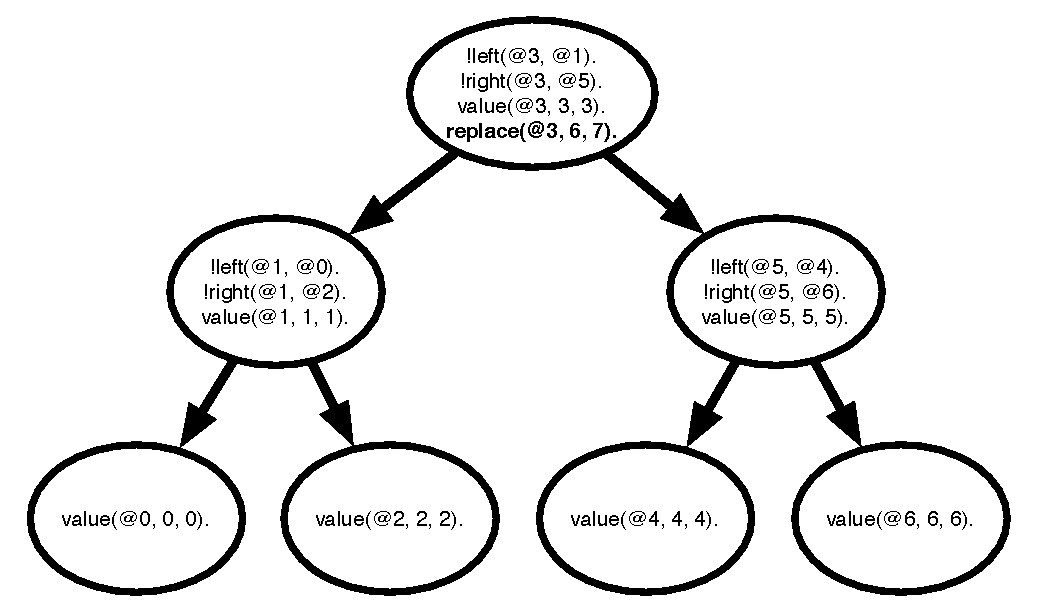
\includegraphics[width=\textwidth]{btree_trace1}
                \caption{Initial database. Replace axiom instantiated at the $@3$ root node.}
                \label{fig:btree_trace1}
        \end{subfigure}%
        ~
        \begin{subfigure}[b]{0.5\textwidth}
                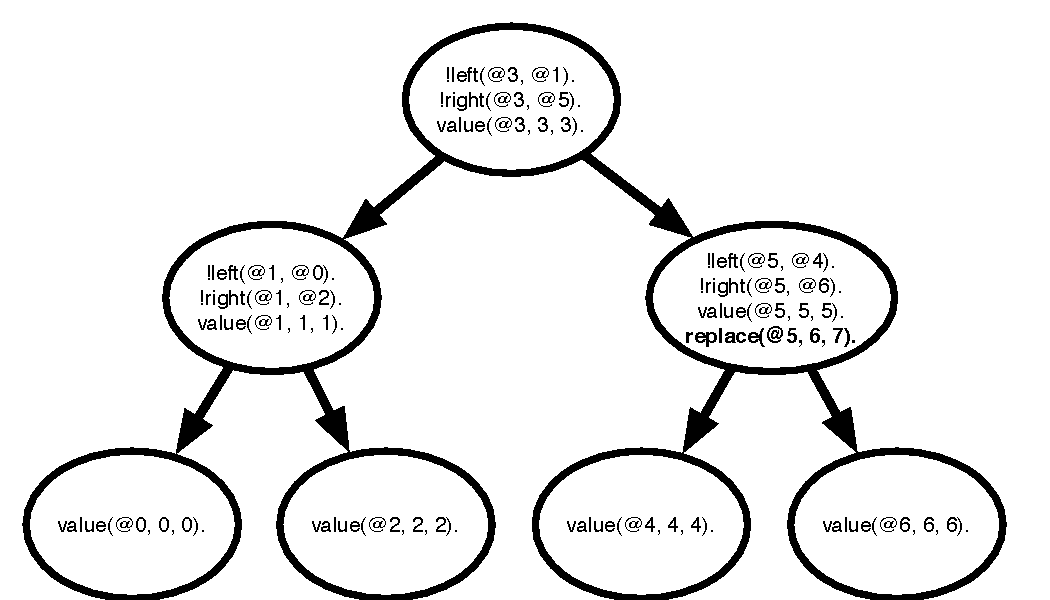
\includegraphics[width=\textwidth]{btree_trace2}
                \caption{After applying rule 3 at node $@3$. Replace fact sent to node $@5$.}
                \label{fig:btree_trace2}
        \end{subfigure}\\
        \begin{subfigure}[b]{0.5\textwidth}
                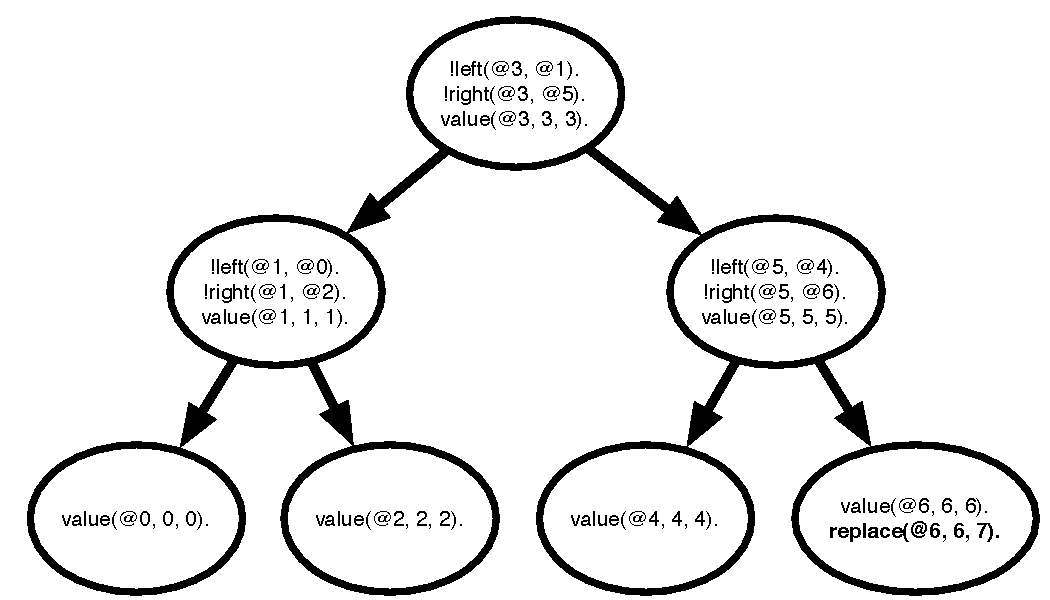
\includegraphics[width=\textwidth]{btree_trace3}
                \caption{After applying rule 3 at node $@5$. Replace fact reaches node $@6$.}
                \label{fig:btree_trace3}
        \end{subfigure}%
        ~
        \begin{subfigure}[b]{0.5\textwidth}
                  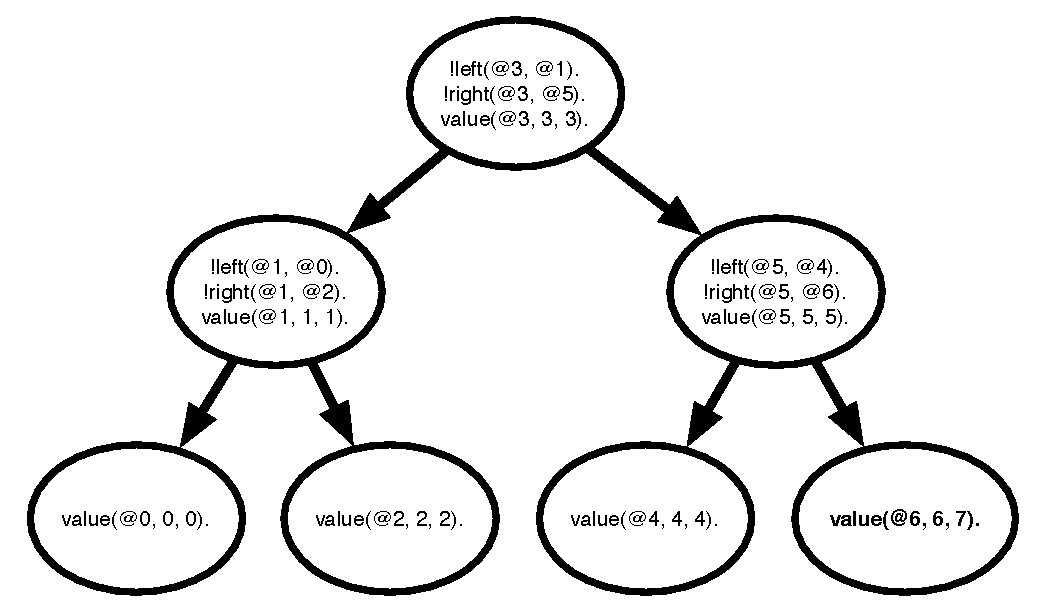
\includegraphics[width=\textwidth]{btree_trace4}
                  \caption{After applying rule 1 (nodes $@5$). Value of key 6 has changed to 7.}
                  \label{fig:btree_trace4}
          \end{subfigure}
        \caption{An execution trace for the binary tree dictionary algorithm.}\label{fig:btree_trace}
\end{figure}

\subsection{Syntax}

\renewcommand{\arraystretch}{1.5}
\begin{table}[]
\centering
\begin{tabular}{ l l c l }
  Program & $Prog$ & $::=$ & $\Sigma, D$ \\
  Set Of Rules & $\Sigma$ & $::=$ & $\cdot \; | \; \Sigma, R$\\
  Database & $D$ & $::=$ & $\Gamma; \Delta$ \\
  Rule & $R$ & $::=$ & $BE \lolli HE \; | \; \forall_{x}. R$ \\
  Body Expression & $BE$ & $::=$ & $L \; | \; P \; | \; C \; | \; BE, BE \; | \; \exists_{x}. BE \; | \; 1$\\
  Head Expression & $HE$ & $::=$ & $L \; | \; P \; | \; HE, HE \; | \; CE \; | \; AE \; | \; 1$\\
  
  Linear Fact & $L$ & $::=$ & $l(\hat{x})$\\
  Persistent Fact & $P$ & $::=$ & $\bang p(\hat{x})$\\
  Constraint & $C$ & $::=$ & $c(\hat{x})$ \\
  
  Comprehension & $CE$ & $::=$ & $\comprehension$ \\
  Aggregate & $AE$ & $::=$ & $\aggregate$ \\
  Aggregate Operation & $A$ & $::=$ & $\mathtt{min} \; | \; \mathtt{max} \; | \; \mathtt{sum} \; | \; \mathtt{count}$ \\
  
  Sub-Head & $SH$ & $::=$ & $L \; | \; P \; | \; SH, SH \; | \; 1$\\
  
  Known Linear Facts & $\Delta$ & $::=$ & $\cdot \; | \; \Delta, l(\hat{t})$ \\
  Known Persistent Facts & $\Gamma$ & $::=$ & $\cdot \; | \; \Gamma, \bang p(\hat{t})$ \\
\end{tabular}
\caption{Abstract syntax of LM.}\label{tbl:ast}
\end{table}
\renewcommand{\arraystretch}{1.0}

Table~\ref{tbl:ast} shows the abstract syntax for rules in LM.
A LM program $Prog$ consists of a set of derivation rules $\Sigma$ and a database $D$.
Each derivation rule $R$ can be written as $BE \lolli HE$ where $BE$ is the body of a rule and
$HE$ is the head. Rules without bodies are allowed in LM and they are called \textit{axioms}. Rules without heads are also allowed.

The body of a rule, $BE$, may contain linear ($L$) and persistent ($P$) \emph{fact expressions}
and constraints ($C$). Fact expressions are template facts that instantiate variables
(from facts in the database). Variables can be used again in the body for matching and
also in the head when instantiating facts. Constraints are boolean expressions that must
be true in order for the rule to be fired. Constraints use variables from fact expressions and are built using a small functional language that includes mathematical operations, boolean operations, external functions and literal values.

The head of a rule, $HE$, contains linear ($L$) and persistent ($P$) \emph{fact templates} which are uninstantiated facts and will derive new facts. The head can also have \emph{comprehensions} ($CE$) and \emph{aggregates} ($AE$). All those expressions
may use all the variables instantiated in the body.

\subsubsection{Comprehensions}

Sometimes we need to consume a linear fact and then immediately generate several facts depending on
the contents of the database. To solve this particular need, we created the concept of comprehensions, which are
sub-rules that are applied with all possible combinations of facts from the database. In a comprehension $\comprehension$,
$\widehat{x}$ is a list of variables, $BE$ is the body of the comprehension and $SH$ is the head.
The body $BE$ is used to generate all possible combinations for the head $SH$, according to the facts
in the database.

The following example illustrates a simple program that uses comprehensions:

\begin{Verbatim}
!edge(@1, @2).
!edge(@1, @3).
iterate(@1).
iterate(A) -o {B | !edge(A, B) | perform(B)}.
\end{Verbatim}

When the rule is fired, we consume \texttt{iterate(@1)} and then generate the comprehension. Here, we iterate through
all the \texttt{edge/2} facts that match \texttt{!edge(@1, B)}, which are: \texttt{!edge(@1, @2)} and \texttt{!edge(@1, @3)}.
For each fact, we derive \texttt{perform(B)}, namely: \texttt{perform(@2)} and \texttt{perform(@3)}.

\subsubsection{Aggregates}

Another useful feature in logic programs is the ability to reduce several facts into a single fact.
In LM we have aggregates ($AE$), a special kind of sub-rule that works very similarly to comprehensions.
In the abstract syntax $\aggregate$, $A$ is the aggregate operation, $\widehat{x}$ is the list of variables
introduced in $BE$, $SH_1$ and $SH_2$ and $y$ is the variable in the body
$BE$ that represents the values to be aggregated using $A$. Like comprehensions,
we use $\widehat{x}$ to try all the combinations of $BE$, but, in addition to deriving $SH_1$ for each combination,
we aggregate the values represented by $y$ and derive $SH_2$ only once using $y$.

To better understand aggregates, let's consider a database with the following facts and a rule:

\begin{Verbatim}
price(@1, 3).
price(@1, 4).
price(@1, 5).
count-prices(@1).
count-prices(A) -o [sum => P | . | price(A, P) | 1 | total(A, P)].
\end{Verbatim}

By applying the rule, we consume \texttt{count-prices(@1)} and
derive the aggregate which consumes all the \texttt{price(@1, P)} facts.
These are summed and \texttt{total(@1,~12)} is derived.  
LM provides several aggregate operations, including the minimum, maximum, sum, and count.

\subsection{Concurrency}

LM is at its core a distributed programming language.
The database of facts can be seen as a graph data structure where each node contains a fraction of the database.
To accomplish this, we force the first argument of each predicate to be typed as a \emph{node}. We then
restrict the derivation rules to only manipulate facts belonging to a single node.
However, the expressions in the head may refer to other nodes, as long as those nodes are instantiated in the body of the rule.

\subsection{Application}

LM has been used to implement several parallel algorithms, including: belief propagation~\cite{Gonzalez+al:aistats09paraml},
belief propagation with residual splash~\cite{Gonzalez+al:aistats09paraml}, PageRank, graph coloring,
N queens, shortest path, diameter estimation, map reduce, game of life, quick-sort, neural network training, among others.
While these results are evidence that LM is a promising language, this paper will only focus on the more formal aspects of our work.

%For the purposes of this paper, we will ignore the distribution aspect of the language and assume that there is a single global database.


\section{Linear Logic}

LM differs greatly from other Datalog-like languages due to the use of linear logic~\cite{Girard95logic:its}. Traditional forward-chaining logic programming languages make only use of classical logic, in which derived facts are true forever. Many ad-hoc extensions~\cite{Liu98extendingdatalog,Ludascher95alogical} have been devised in the past to support state updates in Datalog, but most are extra-logical which makes it harder to reason about programs.
LM uses linear logic as its foundation, therefore state updates are completely natural to the language.

We use a small subset of the original linear logic proof system along with an extension for definitions to improve
the expressiveness of the language. We summarize the connectives used in Table~\ref{table:linear}
and how they relate to LM.

\begin{table*}
   \begin{center}
\resizebox{16cm}{!}{
    \begin{tabular}{ | l | l || l | l | l |}
    \hline
    Connective                   & Description                                      & LM Syntax                                  & LM Place     & LM Example                                  \\ \hline \hline
    $\emph{fact}(\hat{x})$       & Linear facts.                                    & $fact(\hat{x})$                               & Body or Head    & \texttt{path(A, P)}                            \\ \hline
    $\bang \emph{fact}(\hat{x})$ & Persistent facts.                                & $\bang fact(\hat{x})$                         & Body or Head    & \texttt{$\bang$edge(X, Y, W)}                  \\ \hline
    $1$                          & Represents rules with an empty head.             & $1$                                           & Head            & \texttt{1}                                     \\ \hline
    $A \otimes B$                & Connect two expressions.                         & $A, B$                                        & Body and Head   & \texttt{path(A, P), edge(A, B, W)}             \\ \hline
    $\forall x. A$               & To represent variables defined inside the rule.  & Please see $A \lolli B$                       & Rule            & \texttt{path(A, B) $\lolli$ reachable(A, B)}   \\ \hline
    $\exists x. A$               & Instantiates new node variables.                 & $exists \; \widehat{x}. (B)$                  & Head            & \texttt{exists A.(path(A, P))}                 \\ \hline
    $A \lolli B$                 & $\lolli$ means "linearly implies".               & $A \lolli B$                                  & Rule            & \texttt{path(A, B) $\lolli$ reachable(A, B)}   \\
                                 & $A$ is the body and $B$ is the head.             &                                               &                 &                                                \\ \hline
    $\m{def} A. B$               & Extension called definitions.                    & $\{\; \widehat{x} \; | \; A \; | \; B \; \}$  & Head            & \texttt{\{B | !edge(A, B) | visit(B)\}}        \\
                                 & Used for comprehensions and aggregates.          &                                               &                 &                                                \\ \hline
    \end{tabular}
}
\end{center}
\caption{Connectives from Linear Logic used in LM.}
\label{table:linear}
\end{table*}

The sequent calculus for our linear logic fragment is shown in Fig.~\ref{linear_logic}.
The sequent has the form $\Psi ; \seqnocut{\Gamma}{\Delta}{C}$, where $\Psi$ is the typed
term context used in the quantifiers, $\Gamma$ is the multi-set of persistent terms, $\Delta$
is the multi-set of linear terms and $C$ is the term we want to prove.

\begin{figure}[ht]
\[
\infer[\one R]
{\Psi ; \seqnocut{\Gamma}{\cdot}{\one}}
{}
\tab
\infer[\one L]
{\Psi ; \seqnocut{\Gamma}{\Delta, \one}{C}}
{\Psi ; \seqnocut{\Gamma}{\Delta}{C}}
\]

\[
\infer[\with R]
{\Psi ; \seqnocut{\Gamma}{\Delta}{A \with B}}
{\Psi ; \seqnocut{\Gamma}{\Delta}{A} & \seqnocut{\Gamma}{\Delta}{B}}
\tab
\infer[\with L_1]
{\Psi ; \seqnocut{\Gamma}{\Delta, A \with B}{C}}
{\Psi ; \seqnocut{\Gamma}{\Delta, A}{C}}
\tab
\infer[\with L_2]
{\Psi ; \seqnocut{\Gamma}{\Delta, B \with B}{C}}
{\Psi ; \seqnocut{\Gamma}{\Delta, B}{C}}
\]

\[
\infer[\otimes R]
{\Psi ; \seqnocut{\Gamma}{\Delta, \Delta'}{A \otimes B}}
{\Psi ; \seqnocut{\Gamma}{\Delta}{A} & \seqnocut{\Gamma}{\Delta}{B}}
\tab
\infer[\otimes L]
{\Psi ;\seqnocut{\Gamma}{\Delta, A \otimes B}{C}}
{\Psi ; \seqnocut{\Gamma}{\Delta, A, B}{C}}
\]

\[
\infer[\lolli R]
{\Psi ; \seqnocut{\Gamma}{\Delta}{A \lolli B}}
{\Psi ; \seqnocut{\Gamma}{\Delta, A}{B}}
\tab
\infer[\lolli L]
{\seqnocut{\Gamma}{\Delta, \Delta', A \lolli B}{C}}
{\Psi ; \seqnocut{\Gamma}{\Delta}{A} &
   \Psi ; \seqnocut{\Gamma}{\Delta', B}{C}}
\]

\[
\infer[\forall R]
{\Psi ; \seqnocut{\Gamma}{\Delta}{\forall n:\tau. A}}
{\Psi, m:\tau ; \seqnocut{\Gamma}{\Delta}{A\{m/n\}}}
\tab
\infer[\forall L]
{\Psi ; \seqnocut{\Gamma}{\Delta, \forall n:\tau. A}{C}}
{\Psi \vdash M : \tau & \Psi ; \seqnocut{\Gamma}{\Delta, A\{M/n\}}{C}}
\]

\[
\infer[\exists R]
{\Psi ; \seqnocut{\Gamma}{\Delta}{\exists n: \tau. A}}
{\Psi \vdash M : \tau &
   \Psi ; \seqnocut{\Gamma}{\Delta}{A \{M/n\}}}
\tab
\infer[\exists L]
{\Psi ; \seqnocut{\Gamma}{\Delta, \exists n:\tau. A}{C}}
{\Psi, m:\tau ; \seqnocut{\Gamma}{\Delta, A\{m/n\}}{C}}
\]

\[
\infer[\bang R]
{\Psi ; \seqnocut{\Gamma}{\cdot}{\bang A}}
{\Psi ; \seqnocut{\Gamma}{\cdot}{A}}
\tab
\infer[\bang L]
{\Psi ; \seqnocut{\Gamma}{\Delta, \bang A}{C}}
{\Psi ; \seqnocut{\Gamma, A}{\Delta}{C}}
\tab
\infer[\m{copy}]
{\Psi ; \seqnocut{\Gamma, A}{\Delta}{C}}
{\Psi ; \seqnocut{\Gamma, A}{\Delta, A}{C}}
\]

\[
\infer[\m{def} \; R]
{\Psi ; \seqnocut{\Gamma}{\Delta}{\compr{A'}}}
{\Psi ; \seqnocut{\Gamma}{\Delta}{B\theta} &
 A \defeq B & A' \doteq A\theta}
\tab
\infer[\m{def} \; L]
{\Psi ; \seqnocut{\Gamma}{\Delta, \compr{A'}}{C}}
{
   \Psi ; \seqnocut{\Gamma}{\Delta, B\theta}{C} & A \defeq B & A' \doteq A\theta
}
\]
\caption{Linear logic fragment used in LM.}\label{linear_logic}
\end{figure}

Most connectives in our fragment are standard and well known, except for the $\compr{A}$ connective. This
connective is a definition that can be unfolded recursively and is used to logically justify
comprehensions and aggregates. We took inspiration from Baelde's work on least and greatest fixed points
in linear logic~\cite{Baelde:2012:LGF:2071368.2071370}. Baelde's system goes beyond simple recursive
definitions and allows proofs using induction and co-induction in linear logic. Fortunately,
the proof system satisfies cut-elimination which makes it consistent.

\begin{samepage}
In a comprehension, we want to apply an implication as many times as possible matches we can do
using the current database. One way to formally describe comprehensions would be to use persistent
rules that would be used a few times and then would be forgotten. A more reasonable approach is to use
definitions. Given a comprehension $C~=~\{~\widehat{x}~|~A~|~B~\}$ with a body $A$ and a head $B$, then we can build the following definition:
\nopagebreak
\[
\compr{C} \defeq 1 \with ((A \lolli B) \otimes \compr{C})
\]
\end{samepage}

We can unfold $\compr{C}$ to either stop (by selecting $1$) or get a new linear implication $A \lolli B$
to apply the comprehension once. Because we also get another $\compr{C}$ by selecting the right hand side,
the comprehension can be applied again, recursively.

\begin{samepage}
Aggregates work identically, but they need an extra argument to accumulate the aggregated value. If a sum aggregate $C$ has the form $[~\m{sum}~\Rightarrow~y~|~\widehat{x}~|~A~|~B_1~|~B_2~]$, then the definition will be as follows:

\nopagebreak
\[
\compr{C} \; V \defeq (\lambda v. B_2)V \with (\forall x. ((Ax \lolli B_1) \otimes \compr{C} \; (x + V)))
\]
\nopagebreak

The aggregate is initiated as $\compr{C} \; 0$.
\end{samepage}

\section{High Level Dynamic Semantics}


In this section, we are going to present the high level dynamic semantics of LM. Both the high level and the low
level semantics formalize the mechanism of deriving rules and are presented as a sequence of steps, where each step
is a single rule application at the node level. Node communication happens in between execution steps.
Each execution step receives the following as inputs: (1) the node's persistent and linear database and (2) the program's rules.
A step returns the following as outputs: (1) the consumed linear facts, (2) the derived linear facts and
(3) the derived persistent facts.

The high level dynamic semantics (HLD) present a simplified overview of the dynamics of the language that are
closer to the formalism of linear logic present in Fig.~\ref{linear_logic} than a concrete implementation.
Note that both the high level and low level dynamic semantics do not model the use of variable bindings when matching
facts from the database. Unification and variable binding are already well understood in the
literature~\cite{Baader:1994:UT:185705.185711} and they are not necessary for a good understanding of the system.

Starting from the linear logic fragment presented earlier, we consider $\Gamma$ and $\Delta$ the node's database.
Context $\Gamma$ contains atomic formulas representing persistent facts while context $\Delta$ contains atomic formulas
representing linear facts.
We assume that the rules of the program are persistent linear implications with the form
$\bang (A \lolli B)$ that can be apply as many times as needed. However, we do not put the rules in the $\Gamma$
context but in a separate context $\Phi$.

The main idea of HLD is to ignore the right hand side of the sequent calculus
and use inversion on the $\Delta$ and $\Gamma$ contexts so that we only have atomic formulas.
To apply rules we use chaining by focusing on one of the derivation rules in $\Phi$. Note
that during the focusing process we assume that all the atomic formulas (facts) are positive thus the chaining
becomes a forward chaining process.

\subsection{Step}\label{step_hld}

The step judgment picks a node $i$ to execute and then updates all the nodes databases accordingly. We assume the existence of $n$
nodes in the program and partition the global linear context $\Delta$ into $\Delta_1, ..., \Delta_n$ and the global persistent
context $\Gamma$ into $\Gamma_1, ..., \Gamma_n$. After deriving a specific rule at node $i$, the newly derived facts on the right
hand side of the $\doz$judgment may contain facts that need to be sent to other nodes. We assume an automatic partition of derived
facts by analysis of the first argument of each fact.

\[
\infer[\stepz]
{\stepz [\Gamma_1 .. \mid \Gamma_i .. \mid \Gamma_n]; [\Delta_1 .. \mid \Delta_i .. \mid \Delta_n]; \Phi \Longrightarrow [\Gamma_1, \Gamma'_1 .. \mid \Gamma_i, \Gamma'_i .. \mid \Gamma_n, \Gamma'_n]; [\Delta_1, \Delta'_1 .. \mid (\Delta_i - \Xi'), \Delta'_i .. \mid \Delta_n, \Delta'_n]}
{\doz \Gamma_i; \Delta_i; \Phi \rightarrow \Xi'; \Delta'_1, ..., \Delta'_n; \Gamma'_1, ..., \Gamma'_n}
\]

\subsection{Application}

To apply a rule we use the judgment $\doz \Gamma; \Delta; \Phi \rightarrow \Xi'; \Delta'; \Gamma'$.
The input contexts are the following: $\Gamma$, the context of persistent facts; $\Delta$, the context of linear facts; and $\Phi$, the program's rules.
The output contexts are the following: $\Xi'$, the set of consumed linear
resources; $\Delta'$, the set of derived linear facts; and $\Gamma'$, the set of derived persistent
facts. Except $\Phi$, $\Delta'$ and $\Gamma'$, both input and output contexts are directly related to the node that is
executing. The context $\Delta'$ may contain facts that need to be sent to other nodes. 
Note that for the HLD semantics there is no concept of rule priority, so we pick a rule
in a non-deterministic fashion.

The judgment $\az \Gamma ; \Delta ; A \lolli B \rightarrow \Xi'; \Delta'; \Gamma'$ will attempt to apply
the derivation rule $A \lolli B$. To do this, it splits the $\Delta$ context into $\Delta_1$ and $\Delta_2$, namely the
set of linear resources consumed to match the body of the rule ($\Delta_1$) and the remaining linear facts ($\Delta_2$),
respectively. Again, the set of resources needed to match the body of the rule is guessed. The low level dynamic semantics will
deterministically compute $\Delta_1$.

\[
\infer[\doz \m{rule}]
{\doz \Gamma ; \Delta ; R, \Phi \rightarrow \Xi' ; \Delta' ; \Gamma'}
{\az \Gamma ; \Delta ; R \rightarrow \Xi' ; \Delta' ; \Gamma'}
\]

\[
\infer[\az \m{rule}]
{\az \Gamma ; \Delta_1, \Delta_2 ; A \lolli B \rightarrow \Xi' ; \Delta' ; \Gamma'}
{\mz \Gamma ; \Delta_1 \rightarrow A & \dz \Gamma ; \Delta_2; \Delta_1; \cdot ; \cdot ; B \rightarrow \Xi' ; \Delta' ; \Gamma'}
\]

\subsection{Match}

The $\mz \Gamma ; \Delta \rightarrow C$ judgment essentially uses the right ($R$) rules of the original
linear logic fragment in order to match all facts using $\Gamma$ and $\Delta$. We must consume all the linear facts in
the multi-set $\Delta$ when matching $C$. The context $\Gamma$ may be used to match persistent terms in $C$ but such
facts are never consumed since they are persistent.

\[
\infer[\mz 1]
{\mz \Gamma; \cdot \rightarrow 1}
{}
\tab
\infer[\mz p]
{\mz \Gamma; p \rightarrow p }
{}
\tab
\infer[\mz \bang p]
{\mz \Gamma, p; \cdot \rightarrow \bang p}
{}
\]

\[
\infer[\mz \otimes]
{\mz \Gamma; \Delta_1, \Delta_2 \rightarrow A \otimes B}
{\mz \Gamma; \Delta_1 \rightarrow A & \mz \Delta_2 \rightarrow B}
\]

\subsection{Derivation}

The derivation judgment takes the head term of a rule and instantiates all the linear and persistent facts. The form of the judgment
is $\dz \Gamma ; \Delta ; \Xi ; \Gamma_1 ; \Delta_1 ; \Omega \rightarrow \Xi'; \Delta'; \Gamma'$ with the following meaning:

\begin{enumerate}
   \item[$\Gamma$] multi-set of persistent resources in the database;
   \item[$\Delta$] multi-set of linear resources in the database not yet consumed;
   \item[$\Xi$] multi-set of linear resources that have been consumed while matching the body of the rule, matching comprehensions or aggregates;
   \item[$\Gamma_1$] multi-set of persistent facts that have been derived using the current rule;
   \item[$\Delta_1$] multi-set of linear facts that have been derived using the current rule;
   \item[$\Omega$] ordered list contain the terms of the head of rule that still need to be derived. We start with the head of the rule $B$ that is continuously deconstructed to derive all the facts of the rule;
   \item[$\Xi'$] multi-set of consumed linear facts after applying the rule;
   \item[$\Delta'$] multi-set of derived linear facts after applying the rule;
   \item[$\Gamma'$] multi-set of derived persistent facts after applying the rule.
\end{enumerate}

We did not include the aggregates here because they are similar to comprehensions. The main rule to
derive comprehensions is $\dz comp$. It unfolds the comprehension which it can be then either
applied ($\m{derive} \with R$ followed by $\m{derive} \lolli$) or not ($\m{derive} \with L$).
The inference rule $\m{derive} \lolli$ takes the linear implication from the ordered list of head terms and
splits the linear context $\Gamma$ to match the comprehension body and recursively derives the head of the comprehension
and the remaining head terms $\Omega$.
The HLD semantics do not take into account the contents of the database to determine how many times a comprehension
should be applied because the process is entirely non-deterministic.

\[
\infer[\dz p]
{\dz \Gamma ; \Delta ; \Xi ; \Gamma_1 ; \Delta_1 ; p, \Omega \rightarrow \Xi' ; \Delta' ; \Gamma'}
{\dz \Gamma ; \Delta ; \Xi ; \Gamma_1 ; p, \Delta_1 ; \Omega \rightarrow \Xi' ; \Delta' ; \Gamma'}
\tab
\infer[\dz \bang p]
{\dz \Gamma ; \Delta ; \Xi ; \Gamma_1 ; \Delta_1 ; \bang p, \Omega \rightarrow \Xi' ; \Delta' ; \Gamma'}
{\dz \Gamma ; \Delta ; \Xi ; \Gamma_1, p ; \Delta_1 ; \Omega \rightarrow \Xi' ; \Delta' ; \Gamma'}
\]

\[
\infer[\dz \otimes]
{\dz \Gamma ; \Delta ; \Xi ; \Gamma_1 ; \Delta_1 ; A \otimes B, \Omega \rightarrow \Xi' ; \Delta' ; \Gamma'}
{\dz \Gamma ; \Delta ; \Xi ; \Gamma_1 ; \Delta_1 ; A, B, \Omega \rightarrow \Xi' ; \Delta' ; \Gamma'}
\tab
\infer[\dz 1]
{\dz \Gamma ; \Delta ; \Xi ; \Gamma_1; \Delta_1 ; 1, \Omega \rightarrow \Xi' ; \Delta' ; \Gamma'}
{\dz \Gamma ; \Delta ; \Xi ; \Gamma_1; \Delta_1 ; \Omega \rightarrow \Xi' ; \Delta' ; \Gamma'}
\]

\[
\infer[\dz end]
{\dz \Gamma ; \Delta ; \Xi' ; \Gamma' ; \Delta' ; \cdot \rightarrow \Xi' ; \Delta' ; \Gamma'}
{}
\]

\[
\infer[\dz \m{comp}]
{\dz \Gamma ; \Delta ; \Xi ; \Gamma_1 ; \Delta_1 ; \comp A \lolli B, \Omega \rightarrow \Xi' ; \Delta' ; \Gamma'}
{\dz \Gamma ; \Delta ; \Xi ; \Gamma_1 ; \Delta_1 ; 1 \with (A \lolli B \otimes \comp A \lolli B), \Omega \rightarrow \Xi' ; \Delta' ; \Gamma'}
\]

\[
\infer[\dz \lolli]
{\dz \Gamma ; \Delta_a, \Delta_b ; \Xi ; \Gamma_1 ; \Delta_1 ; A \lolli B, \Omega \rightarrow \Xi' ; \Delta' ; \Gamma'}
{\mz \Gamma ; \Delta_a \rightarrow A & \dz \Gamma ; \Delta_b ; \Xi, \Delta_a ; \Gamma_1 ; \Delta_1 ; B, \Omega \rightarrow \Xi' ; \Delta' ; \Gamma'}
\]

\[
\infer[\dz \with L]
{\dz \Gamma ; \Delta ; \Xi ; \Gamma_1 ; \Delta_1 ; A \with B, \Omega \rightarrow \Xi' ; \Delta'; \Gamma'}
{\dz \Gamma ; \Delta ; \Xi ; \Gamma_1 ; \Delta_1 ; A, \Omega \rightarrow \Xi' ; \Delta'; \Gamma'}
\tab
\infer[\dz \with R]
{\dz \Gamma ; \Delta ; \Xi ; \Gamma_1 ; \Delta_1 ; A \with B, \Omega \rightarrow \Xi' ; \Delta' ; \Gamma'}
{\dz \Gamma ; \Delta ; \Xi ; \Gamma_1 ; \Delta_1 ; B, \Omega \rightarrow \Xi' ; \Delta' ; \Gamma'}
\]


\section{Low Level Dynamic Semantics}
The low level dynamic semantics (LLD) removes all the non-deterministic choices in HLD
and makes them deterministic. The new semantics will do the following:

\begin{itemize}
   \item Match rules by priority order;
   \item Determine the set of linear facts needed to match either the body of the rule or the body of comprehensions without guessing;
   \item Apply as many comprehensions as the database allows;
   \item Apply as many aggregates as the database allows.
\end{itemize}

HLD had many different proof trees for a given triplet $\Gamma; \Delta; \Phi$ because HLD allows choices to be made during the inference rules. For instance, in HLD any rule could be selected to be executed. In LLD there is only one proof tree
for a given $\Gamma; \Delta; \Phi$ since there is no guessing involved. LLD semantics present a complete step by step mechanism that is needed to correctly evaluate an LM program. For instance, when LLD tries to apply a rule, it will check if there is enough
facts in the database and backtrack until a rule can be applied.

\begin{theorem}
In LLD, there is only one possible proof for a given $\Gamma; \Delta; \Phi$.
\end{theorem}

\begin{proof}
Inference rules of every judgment in LLD are disjunct, therefore only one inference rule can be applied at any given point in the proof.
\end{proof}

LLD shares exactly the same inputs and outputs as HLD. The first difference between the two systems starts when picking a rule to derive.
Instead of guessing, LLD treats the list of rules as a stack and picks the first rule $R$ to execute (the rule with the highest priority). The remaining rules are stored as a continuation. If $R$ cannot be matched because there is not enough facts in the database,
we backtrack and use the rule continuation to pick the next rule and so on, until one rule can be successfully applied.

\subsection{Continuation Frames}

The most interesting aspect introduced by LLD is the continuation frame. A continuation frame acts as a choice
point that is created during rule matching whenever we try to match a fact expression against the database.
The frame considers all the facts relevant to the expression given the current variable bindings and predicate,
that may or not fail during the remaining matching process.

The frame contains enough state to resume the matching
process at the time of its creation, therefore we can easily backtrack to the choice point and select the next candidate
fact from the database (judgment $\contlld$ or $\contclld$).
We keep all the continuation frames in a continuation stack, so in order to backtrack we update the top frame and
select the next fact candidate to continue the matching process.
If all candidates are exhausted, we pop the top frame and try the next one.

By using this match mechanism, we can determine which facts need to be used to match a rule.
Our LM implementation works like LLD, by iterating over
the available facts at each choice point and then committing to the rule if the matching process
succeeds. However, while the implementation only attempts to match rules with a very high change of success,
LLD is more na\"{i}ve in this aspect because it tries all rules in order.

\subsection{Structure of Continuation Frames}

We have two continuation frame types. One frame is stored when dealing with persistent fact expressions and the other when dealing
with linear fact expressions.

\subsubsection{Persistent Frame}

A persistent frame has the form $[\Gamma'; \Delta; \Xi; \bang p; \Omega; \Lambda; \Upsilon]$, where:

\begin{enumerate}
   \item[$\Delta$] remaining multi-set of linear facts;
   \item[$\Xi$] multi-set of linear facts we have consumed to reach this point;
   \item[$\bang p$] current fact expression that originated this choice point;
   \item[$\Omega$] ordered list of remaining terms needed to match past this choice point;
   \item[$\Lambda$] multi-set of linear fact expressions that we have matched to reach this choice point. All the linear facts that match these terms are located in $\Xi$;
   \item[$\Upsilon$] multi-set of persistent fact expressions that we matched up to this point.
\end{enumerate}

\subsubsection{Linear Frame}

A linear frame has the form $(\Delta; \Delta'; \Xi; p; \Omega; \Lambda; \Upsilon)$, where:

\begin{enumerate}
   \item[$\Delta$] multi-set of linear facts that are not of type $p$ plus all the other $p$'s we have already tried, including the current $p$;
   \item[$\Delta'$] all the other $p$'s we haven't tried yet. It is a multi-set of linear facts;
   \item[$\Xi$] multi-set of linear facts we have consumed to reach this point;
   \item[$p$] current fact expression that originated this choice point;
   \item[$\Omega$] ordered list of remaining terms needed to match past this choice point;
   \item[$\Lambda$] multi-set of linear fact expressions that we have matched to reach this choice point. All the linear facts that match these terms are located in $\Xi$;
   \item[$\Upsilon$] multi-set of persistent fact expressions that we matched up to this point.
\end{enumerate}

\subsection{Step}

The starting inference rule of LLD is identical to the one used in HLD described in \ref{step_hld}.

\[
\infer[\stepz]
{\stepo [\Gamma_1 .. \mid \Gamma_i .. \mid \Gamma_n]; [\Delta_1 .. \mid \Delta_i .. \mid \Delta_n]; \Phi \Longrightarrow [\Gamma_1, \Gamma'_1 .. \mid \Gamma_i, \Gamma'_i .. \mid \Gamma_n, \Gamma'_n]; [\Delta_1, \Delta'_1 .. \mid (\Delta_i - \Xi'), \Delta'_i .. \mid \Delta_n, \Delta'_n]}
{\doo \Gamma_i; \Delta_i; \Phi \rightarrow \Xi'; \Delta'_1, ..., \Delta'_n; \Gamma'_1, ..., \Gamma'_n}
\]

\subsection{Application}

When starting an execution step, we pick the first rule $R_1$ and create a rule continuation with the form $(\Phi, \Delta)$, where $\Phi$
is the stack of remaining rules and $\Delta$ is the starting linear context. Context $\Gamma$ does not need to be saved
because its facts are never deleted.

\[
\infer[\doo \m{rule}]
{\doo \Gamma; \Delta; R_1, \Phi \rightarrow \Xi'; \Delta';\Gamma'}
{\ao \Gamma; \Delta; R_1; (\Phi, \Delta) \rightarrow \Xi';\Delta';\Gamma'}
\]

\[
\infer[\ao \m{rule}]
{\ao \Gamma; \Delta; A \lolli B; R \rightarrow \Xi'; \Delta'; \Gamma'}
{\mo \Gamma; \Delta; \cdot; A; B; \cdot; R \rightarrow \Xi'; \Delta'; \Gamma'}
\]

\subsection{Match}\label{sec:body_match}

The matching judgment uses the form $\mo \Gamma; \Delta; \Xi; \Omega; H; C; R \rightarrow \Xi'; \Delta'; \Gamma'$ where:

\begin{enumerate}
   \item[$\Delta$] multi-set of linear facts still available to complete the matching process;
   \item[$\Xi$] multi-set of linear facts consumed up to this point;
   \item[$\Omega$] ordered list of deconstructed head terms to match;
   \item[$H$] head of the rule;
   \item[$C$] ordered list of frames representing the continuation stack;
   \item[$R$] rule continuation to be used if the current rule fails;
   \item[$\Xi'$] multi-set of consumed linear facts after applying the rule;
   \item[$\Delta'$] multi-set of derived linear facts after applying the rule;
   \item[$\Gamma'$] multi-set of derived persistent facts after applying the rule.
\end{enumerate}

Matching will attempt to use facts from $\Delta$ and $\Gamma$ to match the terms of the body of the rule represented as $\Omega$. During this process continuation frames are pushed into $C$.
If the matching process fails, we use the continuation stack through the $\cont$judgment.

\subsubsection{Linear fact expressions}

The first 4 inference rules are used when the head of $\Omega$ is a linear fact expression $p$: (1) the
continuation stack is empty; (2) the continuation is not empty and a linear continuation frame is at the top;
(3) the continuation stack is not empty and a persistent continuation frame is at the top;
and (4) we cannot find any linear fact in the database that matches $p$. Note that in the first 3 rules,
we find $p_1$ and $\Delta''$ as facts from the database that match $p$ the hidden and partially initialized arguments.
Context $\Delta''$ is stored in the second argument of the new continuation frame but passes along with $\Delta$ since they
have not been consumed yet (just $p_1$).

{\footnotesize
\[
\infer[\mo p~\m{first}]
{\mo \Gamma ; \Delta, p_1, \Delta'' ; \Xi; p, \Omega; H; \cdot; R \rightarrow \Xi'; \Delta'; \Gamma'}
{p_1, \Delta'' \prec p & \mo \Gamma ; \Delta, \Delta''; \Xi, p_1; \Omega; H; (\Delta, p_1; \Delta''; p; \Omega; \Xi; \cdot; \cdot); R \rightarrow \Xi'; \Delta'; \Gamma'}
\]

\[
\infer[\mo p~\m{on}~q]
{\mo \Gamma ; \Delta, p_1, \Delta'' ; \Xi; p, \Omega; H; C_1, C; R \rightarrow \Xi'; \Delta'; \Gamma'}
{p_1, \Delta'' \prec p & \begin{split} C_1 &= (\Delta_{old}; \Delta'_{old}; q; \Omega_{old}; \Xi_{old}; \Lambda; \Upsilon) \\ \mo &\Gamma ; \Delta, \Delta''; \Xi, p_1; \Omega; H; (\Delta, p_1; \Delta''; p; \Omega; \Xi; q, \Lambda; \Upsilon), C_1, C; R \rightarrow \Xi'; \Delta'; \Gamma'\end{split}}
\]


\[
\infer[\mo p~\m{on}~\bang q]
{\mo \Gamma ; \Delta, p_1, \Delta'' ; \Xi; p, \Omega; H; C_1, C; R \rightarrow \Xi'; \Delta'; \Gamma'}
{p_1, \Delta'' \prec p & \begin{split}C_1 &= [\Gamma_{old}; \Delta_{old}; \bang q; \Omega_{old}; \Xi_{old}; \Lambda; \Upsilon] \\ \mo &\Gamma ; \Delta, \Delta''; \Xi, p_1; \Omega; H; (\Delta, p_1; \Delta''; p; \Omega; \Xi; \Lambda; q, \Upsilon), C_1, C; R \rightarrow \Xi'; \Delta'; \Gamma' \end{split}}
\]

\[
\infer[\mo p~\m{fail}]
{\mo \Gamma ; \Delta; \Xi; p, \Omega; H; C; R \rightarrow \Xi'; \Delta'; \Gamma'}
{\Delta \npreceq p & \cont C ; H; R; \Gamma \rightarrow \Xi'; \Delta'; \Gamma'}
\]
}

\subsubsection{Persistent fact expressions}

The next 4 inference rules are used when the head of $\Omega$ contains a persistent fact expression $\bang p$. They are identical
to the previous 4 rules but they deal with the persistent context $\Gamma$.

{\footnotesize
\[
\infer[\mo \bang p~\m{first}]
{\mo \Gamma, p_1, \Gamma'' ; \Delta; \Xi; \bang p, \Omega; H; \cdot; R \rightarrow \Xi'; \Delta'; \Gamma'}
{p_1, \Gamma'' \prec \bang p & \mo \Gamma, p_1, \Gamma'' ; \Delta; \Xi; \Omega; H; [\Gamma''; \Delta; \bang p ; \Omega; \Xi; \cdot; \cdot]; R \rightarrow \Xi'; \Delta'; \Gamma'}
\]

\[
\infer[\mo \bang p~\m{on}~q]
{\mo \Gamma, p_1, \Gamma'' ; \Delta; \Xi; \bang p, \Omega; H; C_1, C; R \rightarrow \Xi'; \Delta'; \Gamma'}
{p_1, \Gamma'' \prec \bang p & \begin{split}C_1 &= (\Delta_{old}; \Delta'_{old}; q; \Omega_{old}; \Xi_{old}; \Lambda; \Upsilon) \\ \mo &\Gamma, p_1, \Gamma'' ; \Delta; \Xi; \Omega; H; [\Gamma''; \Delta; \bang p ; \Omega; \Xi; q, \Lambda; \Upsilon], C_1, C; R \rightarrow \Xi'; \Delta'; \Gamma'\end{split}}
\]


\[
\infer[\mo \bang p~\m{on}~\bang q]
{\mo \Gamma, p_1, \Gamma'' ; \Delta; \Xi; \bang p, \Omega; H; C_1, C; R \rightarrow \Xi'; \Delta'; \Gamma'}
{p_1, \Gamma'' \prec \bang p & \begin{split}C_1 &= [\Gamma_{old}; \Delta_{old}; \bang q; \Omega_{old}; \Xi_{old}; \Lambda; \Upsilon] \\ \mo &\Gamma, p_1, \Gamma'' ; \Delta; \Xi; \Omega; H; [\Gamma''; \Delta; \bang p ; \Omega; \Xi; \Lambda; q, \Upsilon], C_1, C; R \rightarrow \Xi'; \Delta'; \Gamma'\end{split}}
\]

\[
\infer[\mo \bang p~\m{fail}]
{\mo \Gamma ; \Delta; \Xi; \bang p, \Omega; H; C; R \rightarrow \Xi'; \Delta'; \Gamma'}
{\Gamma \npreceq \bang p & \cont C; H; R; \Gamma \rightarrow \Xi'; \Delta'; \Gamma'}
\]
}

\subsubsection{Other expressions}

Finally, we have the inference rule $\mo \otimes$ that deconstructs body terms with $\otimes$ and the $\mo \m{end}$ rule
that terminates the matching process and initiates the derivation of head terms because $\Omega$ is empty.

{\footnotesize
\[
\infer[\mo \otimes]
{\mo \Gamma ; \Delta; \Xi; A \otimes B, \Omega ; H ; C; R \rightarrow \Xi'; \Delta';\Gamma'}
{\mo \Gamma ; \Delta; \Xi; A, B, \Omega; H; C; R \rightarrow \Xi';\Delta';\Gamma'}
\tab
\infer[\mo \m{end}]
{\mo \Gamma ; \Delta; \Xi; \cdot ; H; C; R \rightarrow \Xi'; \Delta'; \Gamma'}
{\done \Gamma ; \Delta; \Xi; \cdot ; H; \cdot \rightarrow \Xi'; \Delta'; \Gamma'}
\]
}

\subsection{Continuation}\label{sec:match_cont}

If the previous matching process fails, we pick the top frame from the stack $C$ and restore the matching process using another fact and/or context. The continuation judgment $\cont C; H; R; \Gamma \rightarrow \Xi'; \Delta'; \Gamma'$ deals with the backtracking process where the meaning of each argument is as follows:

\begin{enumerate}
   \item[$C$] continuation stack;
   \item[$H$] head of the current rule we are executing;
   \item[$R$] next available rules if the current rule does not match.
\end{enumerate}

\subsubsection{Linear continuation frames}

The next two inference rules detect a linear continuation frame on top of the continuation stack. The first rule picks the next
fact candidate $p_1$ from the second argument of the linear frame and updates the frame. Otherwise, if we have no more
candidate facts, we pop the continuation frame and use $\cont$again with the remaining continuation stack.

%{\footnotesize
\[
\infer[\cont p~\m{next}]
{\cont (\Delta; p_1, \Delta''; p, \Omega; \Xi; \Lambda; \Upsilon), C; H; R; \Gamma \rightarrow \Xi'; \Delta'; \Gamma'}
{\mo \Gamma ; \Delta, \Delta''; \Xi, p_1; \Omega; H; (\Delta, p_1; \Delta''; p, \Omega; H; \Xi; \Lambda; \Upsilon), C; R \rightarrow \Xi'; \Delta'; \Gamma'}
\]
%}

%{\footnotesize
\[
\infer[\cont p~\m{no~more}]
{\cont (\Delta; \cdot; p, \Omega; \Xi; \Lambda; \Upsilon), C; H; R; \Gamma \rightarrow \Xi'; \Delta'; \Gamma'}
{\cont C; H; R; \Gamma; \Xi'; \Delta'; \Gamma'}
\]
%}

\subsubsection{Persistent continuation frames} We also have the same two kinds of inference rules for persistent continuation frames.

%{\footnotesize
\[
\infer[\cont \bang p~\m{next}]
{\cont [p_1, \Gamma'; \Delta; \bang p, \Omega; \Xi; \Lambda; \Upsilon], C; H; R; \Gamma \rightarrow \Xi'; \Delta'; \Gamma'}
{\mo \Gamma; \Delta; \Xi; \Omega; H; [\Gamma'; \Delta; \bang p, \Omega; \Xi; \Lambda; \Upsilon], C; R \rightarrow \Xi'; \Delta'; \Gamma'}
\]
%}

%{\footnotesize
\[
\infer[\cont \bang p~\m{no~more}]
{\cont [\cdot; \Delta; \bang p, \Omega; \Xi; \Lambda; \Upsilon], C; H; R; \Gamma \rightarrow \Xi'; \Delta'; \Gamma'}
{\cont C; H; R; \Gamma \rightarrow \Xi'; \Delta'; \Gamma'}
\]
%}

\subsubsection{Empty continuation stack}

Finally, if the continuation stack is empty, we simply force execution to try the next inference rule in $\Phi$.

%{\footnotesize
\[
\infer[\cont \m{next~rule}]
{\cont \cdot; H; (\Phi, \Delta); \Gamma \rightarrow \Xi'; \Delta'; \Gamma'}
{\doo \Gamma; \Delta; \Phi \rightarrow \Xi'; \Delta'; \Gamma'}
\]
%}

\subsection{Derivation}

Once the list of terms $\Omega$ in the $\mo$judgment is exhausted (rule $\mo \m{end}$), we derive the terms of the head of rule.
The derivation judgment uses the form $\done \Gamma; \Delta; \Xi; \Gamma_1; \Delta_1; \Omega \rightarrow \Xi'; \Delta'; \Gamma'$,
where:

\begin{enumerate}
   \item[$\Delta$] multi-set of linear facts we started with minus the linear facts consumed $\Xi$ during the matching of the body of the rule;
   \item[$\Xi$] multi-set of linear facts consumed during the matching of the body of the rule;
   \item[$\Gamma_1$] set of persistent facts derived up to this point in the derivation;
   \item[$\Delta_1$] multi-set of linear facts derived up to this point in the derivation;
   \item[$\Omega$] remaining terms to derive as an ordered list. We start with $B$ if the original rule is $A \lolli B$.
\end{enumerate}

\subsubsection{Fact templates} When deriving either $p$ or $\bang p$ we have the following two inference rules:

{\footnotesize
\[
\infer[\done p]
{\done \Gamma ; \Delta; \Xi; \Gamma_1 ; \Delta_1; p, \Omega \rightarrow \Xi'; \Delta'; \Gamma'}
{\done \Gamma ; \Delta; \Xi; \Gamma_1 ; p, \Delta_1; \Omega \rightarrow \Xi'; \Delta'; \Gamma'}
\tab
\infer[\done \bang p]
{\done \Gamma ; \Delta ; \Xi; \Gamma_1 ; \Delta_1; \bang p, \Omega \rightarrow \Xi'; \Delta'; \Gamma'}
{\done \Gamma ; \Delta ; \Xi; \Gamma_1, p; \Delta_1; \Omega \rightarrow \Xi'; \Delta'; \Gamma'}
\]
}

\subsubsection{Deconstruct head}
The following two inference rules deconstruct the head list $\Omega$ from terms created using either $1$ or $\otimes$.

{\footnotesize
\[
\infer[\done 1]
{\done \Gamma; \Delta; \Xi; \Gamma_1 ; \Delta_1; 1, \Omega \rightarrow \Xi';\Delta';\Gamma'}
{\done \Gamma; \Delta; \Xi; \Gamma_1 ; \Delta_1; \Omega \rightarrow \Xi'; \Delta';\Gamma'}
\tab
\infer[\done \otimes]
{\done \Gamma ; \Delta; \Xi; \Gamma_1; \Delta_1; A \otimes B, \Omega \rightarrow \Xi'; \Delta';\Gamma'}
{\done \Gamma ; \Delta; \Xi; \Gamma_1; \Delta_1; A, B, \Omega \rightarrow \Xi';\Delta';\Gamma'}
\]
}

\subsubsection{Comprehensions} The inference rule $\done \m{comp}$ deals with comprehensions. Comprehensions have the form $A \com B$, where $A$ is the body and $B$ the head of the comprehension. Judgment $\mc$initiates the matching process of the body $A$
of the comprehension (explained in the next section).

{\footnotesize
\[
\infer[\done \m{comp}]
{\done \Gamma; \Delta ; \Xi; \Gamma_1; \Delta_1; A \com B, \Omega \rightarrow \Xi';\Delta';\Gamma'}
{\mc \Gamma; \Delta; \Xi; \Gamma_1; \Delta_1; \cdot; A ; B ; \cdot; \cdot; A \com B; \Omega; \Delta \rightarrow \Xi';\Delta';\Gamma'}
\]
}

\subsubsection{Successful rule} Finally, if the ordered list $\Omega$ is exhausted, then the whole execution process is done.
Note how the output arguments match the input arguments of the $\done$judgment.

{\footnotesize
\[
\infer[\done \m{end}]
{\done \Gamma; \Delta; \Xi; \Gamma_1; \Delta_1; \cdot \rightarrow \Xi; \Delta_1; \Gamma_1}
{}
\]
}


\subsection{Comprehension Match}

The matching process for comprehensions is similar to the process used for matching the body of the rule presented
in Section~\ref{sec:body_match}, however we use two continuation stacks, $C$ and $P$. In $P$, we put all the initial persistent frames
and in $C$ we put the first linear frame and then everything else.

To apply as many comprehensions as the database allows, we
reuse the continuation stacks to backtrack and try all the possible combinations available.
However, in order to reuse the stack, we need to update it by removing all the frames pushed after the first linear continuation frame.
If we tried to use those frames, we would assumed that the linear facts used by the other frames were still in the database, but that
is not true because they have been consumed during the first application of the comprehension.
For example, if the body is $\bang \mathtt{a(X)} \otimes \mathtt{b(X)} \otimes \mathtt{c(X)}$ and the continuation stack has three frames (one per fact), we cannot backtrack to the frame of $\mathtt{c(X)}$
since, at that point, the matching process was assuming that the previous \texttt{b(X)} linear fact was still available.
Moreover, we also need to remove the consumed linear facts from the frames of \texttt{b(X)} and $\bang$\texttt{a(X)} in order to make the stack fully consistent with the new database. We will see later on how to do that.

The full match judgment has the form
$\mc \Gamma; \Delta; \Xi_N; \Gamma_{N1}; \Delta_{N1}; \Xi; \Omega; C; P; AB; \Omega_N; \Delta_N \rightarrow \Xi'; \Delta'; \Gamma'$, where:

\begin{enumerate}
   \item[$\Delta$] multi-set of linear facts remaining up to this point in the matching process;
   \item[$\Xi_N$] multi-set of linear facts used during the matching process of the body of the rule and all the previous comprehensions;
   \item[$\Gamma_{N1}$] set of persistent facts derived up to this point in the head of the rule;
   \item[$\Delta_{N1}$] multi-set of linear facts derived up to this point in the head of the rule;
   \item[$\Xi$] multi-set of linear facts consumed up to this point;
   \item[$\Omega$] ordered list of terms that need to be matched for the comprehension to be applied;
   \item[$C$] continuation stack that contains both linear and persistent frames. The first frame must be linear;
   \item[$P$] initial part of the continuation stack with only persistent frames;
   \item[$AB$] comprehension $A \com B$ that is being matched;
   \item[$\Omega_N$] ordered list of remaining terms of the head of the rule to be derived;
   \item[$\Delta_N$] multi-set of linear facts that were still available after matching the body of the rule and all the previous comprehensions. Note that $\Delta, \Xi = \Delta_N$.
\end{enumerate}

\subsubsection{Linear continuation frames}

The following five inference rules deal with the case when there is a linear fact expression in the body of the comprehension.

{\scriptsize
\[
\infer[\mc p~\m{first}]
{\mc \Gamma; \Delta, p_1, \Delta''; \Xi_N; \Gamma_{N1}; \Delta_{N1}; \cdot; p, \Omega; \cdot; \cdot; AB; \Omega_N; \Delta_N \rightarrow \Xi'; \Delta'; \Gamma'}
{p_1, \Delta'' \prec p & \mc \Gamma; \Delta, \Delta''; \Xi_N; \Gamma_{N1}; \Delta_{N1}; \Xi, p_1; \Omega; (\Delta, p_1; \Delta''; \cdot; p; \Omega; \cdot; \cdot); \cdot; AB; \Omega_N; \Delta_N \rightarrow \Xi'; \Delta'; \Gamma'}
\]

\[
\infer[\mc p~\m{on}~q]
{\mc \Gamma; \Delta, p_1, \Delta''; \Xi_N; \Gamma_{N1}; \Delta_{N1}; \Xi; p, \Omega; C_1, C; P; AB; \Omega_N; \Delta_N \rightarrow \Xi'; \Delta'; \Gamma'}
{p_1, \Delta'' \prec p & \begin{split}C_1 =& (\Delta_{old}; \Delta'_{old}; \Xi_{old}; q; \Omega_{old}; \Lambda; \Upsilon) \\ \mc &\Gamma; \Delta, \Delta''; \Xi_N; \Gamma_{N1}; \Delta_{N1}; \Xi, p_1; \Omega; (\Delta, p_1; \Delta''; \Xi; p; \Omega; q, \Lambda; \Upsilon), C_1, C; P; AB; \Omega_N; \Delta_N \rightarrow \Xi'; \Delta'; \Gamma'\end{split}}
\]


\[
\infer[\mc p~\m{on}~\bang q~C]
{\mc \Gamma; \Delta, p_1, \Delta''; \Xi_N; \Gamma_{N1}; \Delta_{N1}; \Xi; p, \Omega; C_1, C; P; AB; \Omega_N; \Delta_N \rightarrow \Xi'; \Delta'; \Gamma'}
{p_1, \Delta'' \prec p & \begin{split}C_1 &= [\Gamma_{old}; \Delta_{old}; \Xi_{old}; q; \Omega_{old}; \Lambda; \Upsilon] \\ \mc &\Gamma; \Delta, \Delta''; \Xi_N; \Gamma_{N1}; \Delta_{N1}; \Xi, p_1; \Omega; (\Delta, p_1; \Delta''; \Xi; p; \Omega; \Lambda; q, \Upsilon), C_1, C; P; AB; \Omega_N; \Delta_N \rightarrow \Xi'; \Delta'; \Gamma' \end{split}}
\]


\[
\infer[\mc p~\m{on}~\bang q~P]
{\mc \Gamma; \Delta, p_1, \Delta''; \Xi_N; \Gamma_{N1}; \Delta_{N1}; \cdot; p, \Omega; \cdot; P_1, P; AB; \Omega_N; \Delta_N \rightarrow \Xi'; \Delta'; \Gamma'}
{p_1, \Delta'' \prec p & \begin{split}\\ P_1 &= [\Gamma_{old}; \Delta_N; \cdot; q; \Omega_{old}; \cdot; \Upsilon]\\ \Delta_N &= \Delta, p_1, \Delta'' \\ \mc &\Gamma; \Delta, \Delta''; \Xi_N; \Gamma_{N1}; \Delta_{N1}; p_1; \Omega; (\Delta, p_1; \Delta''; \cdot; p; \Omega; \cdot; q, \Upsilon); P_1, P; AB; \Omega_N; \Delta_N \rightarrow \Xi'; \Delta'; \Gamma'\end{split}}
\]


\[
\infer[\mc p~\m{fail}]
{\mc \Gamma; \Delta; \Xi_N; \Gamma_{N1}; \Delta_{N1}; \Xi; p, \Omega; C; P; AB; \Omega_N; \Delta_N \rightarrow \Xi'; \Delta'; \Gamma'}
{\Delta \npreceq p & \contc \Gamma; \Delta_N; \Xi_N; \Gamma_{N1}; \Delta_{N1}; C; P; AB; \Omega_N \rightarrow \Xi'; \Delta'; \Gamma'}
\]
}

\subsubsection{Persistent continuation frames}

If we find a persistent fact expression, the inference rules are similar to the previous ones.

{\scriptsize
\[
\infer[\mc \bang p~\m{first}]
{\mc \Gamma, p_1, \Gamma''; \Delta_N; \Xi_N; \Gamma_{N1}; \Delta_{N1}; \cdot; \bang p, \Omega; \cdot; \cdot; AB; \Omega_N; \Delta_N \rightarrow \Xi'; \Delta'; \Gamma'}
{p_1, \Gamma'' \prec \bang p & \mc \Gamma, p_1, \Gamma''; \Delta_N; \Xi_N; \Gamma_{N1}; \Delta_{N1}; \cdot; \Omega; \cdot; [\Gamma''; \Delta_N; \cdot; \bang p; \cdot; \Omega; \cdot; \cdot]; AB; \Omega_N; \Delta_N \rightarrow \Xi'; \Delta'; \Gamma'}
\]

\[
\infer[\mc \bang p~\m{on}~\bang q~P]
{\mc \Gamma, p_1, \Gamma''; \Delta_N; \Xi_N; \Gamma_{N1}; \Delta_{N1}; \cdot; \bang p, \Omega; \cdot; P_1, P; AB; \Omega_N; \Delta_N \rightarrow \Xi'; \Delta'; \Gamma'}
{p_1, \Gamma'' \prec \bang p & \begin{split}P_1 &= [\Gamma_{old}; \Delta_N; \cdot; \bang q; \Omega_{old}; \cdot; \Upsilon] \\ \mc &\Gamma, p_1, \Gamma''; \Delta_N; \Xi_N; \Gamma_{N1}; \Delta_{N1}; \cdot; \Omega; [\Gamma''; \Delta_N; \cdot; \bang p; \cdot; \Omega; \cdot; q, \Upsilon], P_1, P; AB; \Omega_N; \Delta_N \rightarrow \Xi'; \Delta'; \Gamma'\end{split}}
\]


\[
\infer[\mc \bang p~\m{on}~\bang q~C]
{\mc \Gamma, p_1, \Gamma''; \Delta; \Xi_N; \Gamma_{N1}; \Delta_{N1}; \Xi; \bang p, \Omega; C_1, C; P; AB; \Omega_N; \Delta_N \rightarrow \Xi'; \Delta'; \Gamma'}
{p_1, \Gamma'' \prec \bang p & \begin{split}C_1 &= [\Gamma_{old}; \Delta_{old}; \Xi_{old}; \bang q; \Omega_{old}; \Lambda; \Upsilon] \\ \mc & \Gamma, p_1, \Gamma''; \Delta; \Xi_N; \Gamma_{N1}; \Delta_{N1}; \Xi; \Omega; [\Gamma''; \Delta; \Xi; \bang p; \cdot; \Omega; \Lambda; q, \Upsilon], C_1, C; P; AB; \Omega_N; \Delta_N \rightarrow \Xi'; \Delta'; \Gamma' \end{split}}
\]


\[
\infer[\mc \bang p~\m{on}~q~C]
{\mc \Gamma, p_1, \Gamma''; \Delta; \Xi_N; \Gamma_{N1}; \Delta_{N1}; \Xi; \bang p, \Omega; C_1, C; P; AB; \Omega_N; \Delta_N \rightarrow \Xi'; \Delta'; \Gamma'}
{p_1, \Gamma'' \prec \bang p & \begin{split}C_1 &= (\Delta_{old}; \Delta'_{old}; \Xi_{old}; q; \Omega_{old}; \Lambda; \Upsilon) \\ \mc &\Gamma, p_1, \Gamma''; \Delta; \Xi_N; \Gamma_{N1}; \Delta_{N1}; \Xi; \Omega; [\Gamma''; \Delta; \Xi; \bang p; \cdot; \Omega; \Lambda, q; \Upsilon], C_1, C; P; AB; \Omega_N; \Delta_N \rightarrow \Xi'; \Delta'; \Gamma'\end{split}}
\]

\[
\infer[\mc \bang p~\m{fail}]
{\mc \Gamma; \Delta; \Xi_N; \Gamma_{N1}; \Delta_{N1}; \Xi; \bang p, \Omega; C; P; AB; \Omega_N; \Delta_N \rightarrow \Xi'; \Delta; \Gamma'}
{\Gamma \npreceq \bang p & \contc \Gamma; \Delta_N; \Xi_N; \Gamma_{N1}; \Delta_{N1}; C; P; AB; \Omega_N \rightarrow \Xi'; \Delta'; \Gamma'}
\]
}

\subsubsection{Deconstruct body}

The inference rules for deconstructing the body of the comprehension, including the connectives $\otimes$ and $1$, are shown next.

{\scriptsize
\[
\infer[\mc \otimes]
{\mc \Delta; \Xi_N; \Delta_{N1}; \Xi; X \otimes Y, \Omega; C; P; AB; \Omega_N; \Delta_N \rightarrow \Xi'; \Delta'}
{\mc \Delta; \Xi_N; \Delta_{N1}; \Xi; X, Y, \Omega; C; P; AB; \Omega_N; \Delta_N \rightarrow \Xi'; \Delta'}
\]

\[
\infer[\mc 1]
{\mc \Delta; \Xi_N; \Delta_{N1}; \Xi; 1, \Omega; C; P; AB; \Omega_N; \Delta_N \rightarrow \Xi'; \Delta'}
{\mc \Delta; \Xi_N; \Delta_{N1}; \Xi; \Omega; C; P; AB; \Omega_N; \Delta_N \rightarrow \Xi'; \Delta'}
\]
}

\subsubsection{Successful match}

Finally, when there is no more body terms to process, we initiate the process of the updating the continuation stack (with $\dall$) followed
by deriving the head of the comprehension.

{\scriptsize
\[
\infer[\mc \m{end}]
{\mc \Gamma; \Delta; \Xi_N; \Gamma_{N1}; \Delta_{N1}; \Xi; \cdot; C; P; AB; \Omega_N; \Delta_N \rightarrow \Xi'; \Delta'; \Gamma'}
{\dall \Gamma; \Xi_N; \Gamma_{N1}; \Delta_{N1}; \Xi; C; P; AB; \Omega_N; \Delta_N \rightarrow \Xi'; \Delta'; \Gamma'}
\]
}

\subsection{Continuation Stack Update}

As we said before, to update the continuation stacks, we need remove to all the frames except the first linear frame and remove the consumed linear facts from the remaining frames so that they are still valid for the next application of the comprehension.
The judgment that updates the stack has the form $\dall \Gamma; \Xi_N; \Gamma_{N1}; \Delta_{N1}; \Xi; C; P; AB; \Omega_N; \Delta_N \rightarrow \Xi'; \Delta'; \Gamma'$, where:

\begin{enumerate}
   \item[$\Xi_N$] multi-set of linear facts used during the matching process of the body of the rule and all the previous comprehensions;
   \item[$\Gamma_{N1}$] set of persistent facts derived by the head of the rule and all the previous comprehensions;
   \item[$\Delta_{N1}$] multi-set of linear facts derived by the head of the rule and all the previous comprehensions;
   \item[$\Xi$] multi-set of linear facts consumed by the previous application of the comprehension;
   \item[$C, P$] continuation stacks for the comprehension;
   \item[$AB$] comprehension $A \com B$ that is being computed;
   \item[$\Omega_N$] ordered list of remaining terms of the head of the rule to be derived;
   \item[$\Delta_N$] multi-set of linear facts that were still available after matching the body of the rule and all the previous comprehensions.
\end{enumerate}

\subsubsection{Remove linear continuation frames}

To remove all linear continuation frames except the first one, we simply go through all the frames in the stack $C$ with $\dall \m{more}$
until only one frame remains. This frame is then updated using $\dall \m{end~linear}$ by removing the linear facts $\Xi$ consumed
during the last application of the comprehension.

{\footnotesize
\[
\infer[\dall \m{end~linear}]
{\dall \Gamma; \Xi_N; \Gamma_{N1}; \Delta_{N1}; \Xi; (\Delta_x; \Delta''; \cdot; p; \Omega; \cdot; \Upsilon); P;  AB; \Omega_N; \Delta_N \rightarrow \Xi'; \Delta'; \Gamma'}
{\begin{split}\strans &\Xi; P; P' \\ \dc \Gamma; \Xi_N, \Xi; \Gamma_{N1}; \Delta_{N1}; (\Delta_x - \Xi; \Delta'' - \Xi; \cdot;& p; \Omega; \cdot; \Upsilon) ; P' ; AB; \Omega_N; (\Delta_N - \Xi) \rightarrow \Xi'; \Delta'; \Gamma'\end{split}}
\]

\[
\infer[\dall \m{more}]
{\dall \Gamma; \Xi_N; \Gamma_{N1}; \Delta_{N1}; \Xi; \_, X, C; P; AB; \Omega_N; \Delta_N \rightarrow \Xi'; \Delta'; \Gamma'}
{\dall \Gamma; \Xi_N; \Gamma_{N1}; \Delta_{N1}; \Xi; X, C; P; AB; \Omega_N; \Delta_N \rightarrow \Xi'; \Delta'; \Gamma'}
\]

\[
\infer[\dall \m{end~empty}]
{\dall \Gamma; \Xi_N; \Gamma_{N1}; \Delta_{N1}; \Xi; \cdot; P;  AB; \Omega_N; \Delta_N \rightarrow \Xi'; \Delta'; \Gamma'}
{\begin{split}\strans &\Xi; P; P' \\ \dc \Gamma; \Xi_N, \Xi; \Gamma_{N1}; \Delta_{N1}; \cdot ; P' ; &AB; \Omega_N; (\Delta_N - \Xi) \rightarrow \Xi'; \Delta'; \Gamma'\end{split}}
\]
}

\subsubsection{Transform persistent continuation frames}

Finally, we also need to subtract the consumed facts in $\Xi$ from the second argument of every persistent continuation frame.
We have an auxiliary judgment $\strans \Xi; P; P'$ where $\Xi$ is the multi-set of consumed linear facts, $P$ is the persistent continuation
stack and $P'$ is the stack $P$ after the update.

{\footnotesize
\[
\infer[\strans]
{\strans \Xi; [\Gamma'; \Delta_N; \cdot; \bang p; \Omega; \cdot; \Upsilon], P; [\Gamma'; \Delta_N - \Xi; \cdot; \bang p, \Omega; \cdot; \Upsilon], P'}
{\strans \Xi; P; P'}
\tab
\infer[\strans \m{end}]
{\strans \Xi; \cdot; \cdot}
{\strans \Xi; \cdot; \cdot}
\]
}

\subsection{Comprehension Continuation}

If the comprehension match fails, we need to backtrack to the previous frame and restore the matching process at that point. The judgment used to backtrack is similar to the one presented in Section~\ref{sec:match_cont} and has the form $\contc \Gamma; \Delta_N; \Xi_N; \Delta_{N1}; C; P; AB; \Omega_N \rightarrow \Xi'; \Delta'; \Gamma'$, where:

\begin{enumerate}
   \item[$\Delta_N$] multi-set of linear facts still available after matching the body of the rule;
   \item[$\Xi_N$] multi-set of linear facts used to match the body of the rule and all the previous comprehensions;
   \item[$\Gamma_{N1}$] set of persistent facts derived by the head of the rule and all the previous comprehensions;
   \item[$\Delta_{N1}$] multi-set of linear facts derived by the head of the rule and all the previous comprehensions;
   \item[$C, P$] continuation stacks;
   \item[$AB$] comprehension $A \com B$ that is executing;
   \item[$\Omega_N$] ordered list of remaining terms of the head of the rule to be derived.
\end{enumerate}

\subsubsection{Using C stack}

The following 4 inference rules use the $C$ stack, the stack where the first continuation frame is linear, to perform backtracking.

{\small
\[
\infer[\contc \m{next}~C~p]
{\contc \Gamma; \Delta_N; \Xi_N; \Gamma_{N1}; \Delta_{N1}; (\Delta; p_1, \Delta''; \Xi; p; \Omega; \Lambda; \Upsilon), C; P; AB; \Omega_N \rightarrow \Xi'; \Delta'; \Gamma'}
{\mc \Gamma; \Delta; \Xi_N; \Gamma_{N1}; \Delta_{N1}; \Xi; \Omega; (\Delta, p_1; \Delta''; \Xi; p; \Omega; \Lambda; \Upsilon), C; P; AB; \Omega_N; \Delta_N \rightarrow \Xi'; \Delta'; \Gamma'}
\]

\[
\infer[\contc \m{next}~C~\bang p]
{\contc \Gamma; \Delta_N; \Xi_N; \Gamma_{N1}; \Delta_{N1}; [p_1, \Gamma'; \Delta; \Xi; \bang p; \Omega; \Lambda; \Upsilon], C; P; AB; \Omega_N \rightarrow \Xi'; \Delta'; \Gamma'}
{\mc \Gamma; \Delta; \Xi_N; \Gamma_{N1}; \Delta_{N1}; \Xi; \Omega; [\Gamma'; \Delta; \Xi; \bang p; \Omega; \Lambda; \Upsilon], C; P; AB; \Omega_N; \Delta_N \rightarrow \Xi'; \Delta'; \Gamma'}
\]

\[
\infer[\contc \m{next}~C~\m{empty}~p]
{\contc \Gamma; \Delta_N; \Xi_N; \Gamma_{N1}; \Delta_{N1}; (\Delta; \cdot; \Xi; p; \Omega; \Lambda; \Upsilon), C; P; AB; \Omega_N \rightarrow \Xi'; \Delta'; \Gamma'}
{\contc \Gamma; \Delta_N; \Xi_N; \Gamma_{N1}; \Delta_{N1}; C; P; AB; \Omega_N \rightarrow \Xi'; \Delta'; \Gamma'}
\]

\[
\infer[\contc \m{next}~C~\m{empty}~\bang p]
{\contc \Gamma; \Delta_N; \Xi_N; \Gamma_{N1}; \Delta_{N1}; [\cdot; \Delta; \Xi; \bang p; \Omega; \Lambda; \Upsilon], C; P; AB; \Omega_N \rightarrow \Xi'; \Delta'; \Gamma'}
{\contc \Gamma; \Delta_N; \Xi_N; \Gamma_{N1}; \Delta_{N1}; C; P; AB; \Omega_N \rightarrow \Xi'; \Delta'; \Gamma'}
\]
}

\subsubsection{Using P stack}

The following 2 inference rules use the $P$ stack instead, the stack where all continuation frames are persistent.

{\small
\[
\infer[\contc \m{next}~P~\bang p]
{\contc \Gamma; \Delta_N; \Xi_N; \Gamma_{N1}; \Delta_{N1}; \cdot; [p_1, \Gamma'; \Delta_N; \cdot; \bang p; \Omega; \cdot; \Upsilon], P; AB; \Omega_N \rightarrow \Xi'; \Delta'; \Gamma'}
{\mc \Gamma; \Delta_N; \Xi_N; \Gamma_{N1}; \Delta_{N1}; \cdot; \Omega; \cdot; [\Gamma'; \Delta_N; \cdot; \bang p; \Omega; \cdot; \Upsilon], P; AB; \Omega_N; \Delta_N \rightarrow \Xi'; \Delta'; \Gamma'}
\]

\[
\infer[\contc \m{next}~P~\m{empty}~\bang p]
{\contc \Gamma; \Delta_N; \Xi_N; \Gamma_{N1}; \Delta_{N1}; \cdot; [\cdot; \Delta_N; \cdot; \bang p; \Omega; \cdot; \Upsilon], P; AB; \Omega_N \rightarrow \Xi'; \Delta'; \Gamma'}
{\contc \Gamma; \Delta_N; \Xi_N; \Gamma_{N1}; \Delta_{N1}; \cdot; P; AB; \Omega_N \rightarrow \Xi'; \Delta'; \Gamma'}
\]
}

\subsubsection{Comprehension done}

If both the $C$ and $P$ stacks are empty, we are unable to backtrack and thus unable to continue deriving the comprehension.
We next derive the remaining head terms in $\Omega$.

{\small
\[
\infer[\contc \m{end}]
{\contc \Gamma; \Delta_N; \Xi_N; \Gamma_{N1}; \Delta_{N1}; \cdot; \cdot; AB; \Omega \rightarrow \Xi'; \Delta'; \Gamma'}
{\done \Gamma; \Delta_N; \Xi_N; \Gamma_{N1}; \Delta_{N1}; \Omega \rightarrow \Xi'; \Delta'; \Gamma'}
\]
}

\subsection{Comprehension Derivation}

After updating the continuation stacks, we then derive the head of the comprehension. The judgment has the form $\dc \Gamma; \Xi; \Gamma_1; \Delta_1; \Omega; C; P; AB; \Omega_N; \Delta_N \rightarrow \Xi'; \Delta'; \Gamma'$, where:

\begin{enumerate}
   \item[$\Xi$] multi-set of linear facts consumed both by the body of the rule and previous comprehension applications;
   \item[$\Gamma_1$] set of persistent facts derived by the head of the rule, previous comprehensions and current derivation;
   \item[$\Delta_1$] multi-set of linear facts derived by the head of the rule, previous comprehensions and current derivation;
   \item[$\Omega$] ordered list of terms to derive;
   \item[$C, P$] new continuation stacks;
   \item[$AB$] comprehension $A \com B$ that is being executed;
   \item[$\Omega_N$] ordered list of remaining terms of the head of the rule to be derived;
   \item[$\Delta_N$] multi-set of remaining linear facts that can be used for the next comprehension applications.
\end{enumerate}

{\footnotesize
\[
\infer[\dc p]
{\dc \Gamma; \Xi; \Gamma_1; \Delta_1; p, \Omega; C; P; AB; \Omega_N; \Delta_N \rightarrow \Xi'; \Delta'; \Gamma'}
{\dc \Gamma; \Xi; \Gamma_1; \Delta_1, p; \Omega; C; P; AB; \Omega_N; \Delta_N \rightarrow \Xi'; \Delta'; \Gamma'}
\]

\[
\infer[\dc \bang p]
{\dc \Gamma; \Xi; \Gamma_1; \Delta_1; \bang p, \Omega; C; P; AB; \Omega_N; \Delta_N \rightarrow \Xi'; \Delta'; \Gamma'}
{\dc \Gamma; \Xi; \Gamma_1, p; \Delta_1; \Omega; C; P; AB; \Omega_N; \Delta_N \rightarrow \Xi'; \Delta'; \Gamma'}
\]

\[
\infer[\dc \otimes]
{\dc \Gamma; \Xi; \Gamma_1; \Delta_1; A \otimes B, \Omega; C; P; AB; \Omega_N; \Delta_N \rightarrow \Xi'; \Delta';\Gamma'}
{\dc \Gamma; \Xi; \Gamma_1; \Delta_1; A, B, \Omega; C; P; AB; \Omega_N; \Delta_N \rightarrow \Xi'; \Delta';\Gamma'}
\]

\[
\infer[\dc 1]
{\dc \Gamma; \Xi; \Gamma_1; \Delta_1; 1, \Omega; C; P; AB; \Omega_N; \Delta_N \rightarrow \Xi'; \Delta';\Gamma'}
{\dc \Gamma; \Xi; \Gamma_1; \Delta_1; \Omega; C; P; AB; \Omega_N; \Delta_N \rightarrow \Xi'; \Delta';\Gamma'}
\]
}

The last derivation rule is activated whenever the $\Omega$ is empty. We use the $\contc$judgment to reuse the continuation stack
and try the next combination for the comprehension.

{\footnotesize
\[
\infer[\dc \m{end}]
{\dc \Gamma; \Xi; \Gamma_1; \Delta_1; \cdot; C; P; AB; \Omega_N; \Delta_N \rightarrow \Xi'; \Delta'; \Gamma'}
{\contc \Gamma; \Delta_N; \Xi; \Gamma_1; \Delta_1; C; P; AB; \Omega_N \rightarrow \Xi'; \Delta'; \Gamma'}
\]
}

\section{Soundness Proof}

Now that we have presented both the HLD and LLD semantics, we are in position to start building our soundness theorem.
The soundness theorem proves that if a rule was successfully derived in the LLD semantics then it can also be derived
in the HLD semantics. Since the HLD semantics are so close to linear logic, we prove that our language has a determined, correct,
proof search behavior when executing programs. However, the completeness theorem cannot be proven since LLD lacks the non-determinism
inherent in HLD.


First and foremost, we need to prove some auxiliary theorems and definitions that will be used during the soundness theorem.

\subsection{Term Equivalence}
The first definition defines the equality between two multi-sets of terms.
Two multi-sets $A$ and $B$ are equal, $\feq{A}{B}$, when they have the same constituent atoms.

{\small
\[
\infer[\equiv p]
{\feq{p, A}{p, B}}
{\feq{A}{B}}
\tab
\infer[\equiv \bang p]
{\feq{\bang p, A}{\bang p, B}}
{\feq{A}{B}}
\tab
\infer[\equiv 1~L]
{\feq{1, A}{B}}
{\feq{A}{B}}
\tab
\infer[\equiv 1~R]
{\feq{A}{1, B}}
{\feq{A}{B}}
\]

\[
\infer[\equiv \cdot]
{\feq{\cdot}{\cdot}}
{}
\tab
\infer[\equiv \otimes~L]
{\feq{A \otimes B, C}{D}}
{\feq{A, B, C}{D}}
\tab
\infer[\equiv \otimes~R]
{\feq{A}{B \otimes C, D}}
{\feq{A}{B, C, D}}
\]
}

\begin{theorem}[Match equivalence]
If two multi-sets are equivalent, $\feq{A_1, ..., A_n}{B_1, ..., B_m}$, and we can match $A_1 \otimes ... \otimes A_n$ in HLD such that $\mz \Gamma ; \Delta \rightarrow A_1 \otimes ... \otimes A_n$ then $\mz \Gamma; \Delta \rightarrow B_1 \otimes ... \otimes B_m$ is also true.
\end{theorem}
\begin{proof}
By straightforward induction on the first assumption.
\end{proof}

\subsection{Well-Formed Continuation Frames}
Given a body $A$ that we want to match, the starting linear context $\Delta_{N}$ and the persistent context $\Gamma$, we want to
make sure that the frames used are always well-formed in relation to $A$ and the contexts.

\begin{definition}[Well-formed frame]

Given a triplet $A; \Gamma; \Delta_{N}$ where $A$ is a term, $\Gamma$ is a multi-set of persistent resources and $\Delta_{N}$ a multi-set of linear resources we say that a frame $f$ is well-formed iff:

\begin{enumerate}
   \item Linear frame $f = (\Delta, p_1; \Delta'; \Xi_1, ..., \Xi_m; p; \Omega_1, ..., \Omega_n; \Lambda_1, ..., \Lambda_m; \Upsilon_1, ..., \Upsilon_k)$
   \begin{enumerate}
      \item $\feq{p, \Omega_1, ..., \Omega_n, \Lambda_1, ..., \Lambda_m, \Upsilon_1, ..., \Upsilon_k}{A}$ (the remaining terms and already matched terms are equivalent to the initial body $A$);
      \item $\mz \Xi_1, ..., \Xi_m \rightarrow \Lambda_1 \otimes ... \otimes \Lambda_m$ and $\mz \Xi_i \rightarrow \Lambda_i$ for every $i$;
      \item $\Delta, \Delta', \Xi, p_1 = \Delta_{N}$ (available facts, candidate facts for $p$, consumed facts and the linear fact used for $p$, respectively, are the same as the initial $\Delta_{N}$);
      \item $\mz \Gamma; \cdot \rightarrow \Upsilon_1 \otimes ... \otimes \Upsilon_k$.
   \end{enumerate}
   \item Persistent frame $f = [\Gamma'; \Delta; \Xi_1, ..., \Xi_m; \bang p; \Omega_1, ..., \Omega_n; \Lambda_1, ..., \Lambda_m; \Upsilon_1, ..., \Upsilon_k]$
      \begin{enumerate}
         \item $\feq{\bang p, \Omega_1, ..., \Omega_n, \Lambda_1, ..., \Lambda_m, \Upsilon_1, ..., \Upsilon_k}{A}$;
         \item $\mz \Xi_1, ..., \Xi_m \rightarrow \Lambda_1 \otimes ... \otimes \Lambda_m$ and $\mz \Xi_i \rightarrow \Lambda_i$ for every $i$;
         \item $\Delta, \Xi = \Delta_{N}$;
         \item $\mz \Gamma; \cdot \rightarrow \bang p \otimes \Upsilon_1 \otimes ... \otimes \Upsilon_k$;
         \item $\Gamma' \subset \Gamma$ (remaining candidates are a subset of $\Gamma$).
      \end{enumerate}
\end{enumerate}
\end{definition}

\begin{definition}[Well-formed stack]
A continuation stack $C$ is well-formed iff every frame is well-formed.
\end{definition}

Given the previous definitions, we can now define what it means for a matching judgment to be well-formed.

\begin{definition}[Well-formed body match]

$\mo \Gamma; \Delta; \Xi; \Omega; H; C; R \rightarrow \Xi'; \Delta'; \Gamma'$ is well-formed in relation to a triplet $A; \Gamma; \Delta_{N}$ iff:

\begin{enumerate}
   \item $\Delta, \Xi = \Delta_{N}$
   \item $C$ is well-formed in relation to $A; \Gamma; \Delta_{N}$ and:
   \begin{enumerate}
      \item If $C = \cdot$
   
      $\feq{\Omega}{A}$.
   
      \item Else if $C = (\Delta_a, p_1; \Delta_b; \Xi''; p; \Omega'; \Lambda_1, ..., \Lambda_m; \Upsilon_1, ..., \Upsilon_k), C'$
   
      \begin{enumerate}
         \item $\feq{\Omega'}{\Omega}$;
         \item $p_1 \in \Xi$ and $\mz \Gamma; p_1 \rightarrow p$;
         \item $\Xi = \Xi'', p_1$;
         \item $\Delta = \Delta_a, \Delta_b$.
      \end{enumerate}
      \item Else if $C = [\Gamma'; \Delta''; \Xi''; \bang p; \Omega'; \Lambda_1, ..., \Lambda_m; \Upsilon_1, ..., \Upsilon_k], C'$
      \begin{enumerate}
         \item $\feq{\Omega}{\Omega'}$;
         \item $\Xi = \Xi''$;
         \item $\Delta = \Delta''$.
      \end{enumerate}
   \end{enumerate}
\end{enumerate}

\end{definition}

\begin{definition}[Well-formed comprehension match]
$\mc \Gamma; \Delta; \Xi_N; \Gamma_{N1}; \Delta_{N1}; \Xi; \Omega; C; P; A \com B; \Omega_N; \Delta_N \rightarrow \Xi'; \Delta'; \Gamma'$ is well-formed in relation to a triplet $A; \Gamma; \Delta_{N}$ iff:

\begin{enumerate}
   \item $P$ is only composed of persistent frames.
   \item $C$ is composed of either linear or persistent frames, but the first frame is linear.
   \item $\Delta, \Xi = \Delta_{N}$
   \item $C$ and $P$ are well-formed in relation to $A; \Gamma; \Delta_{N}$ and:
   \begin{enumerate}
      \item If $C = \cdot$ and $P = \cdot$
      
      $\feq{\Omega}{A}$.
      
      \item Else if $C = \cdot$ and $P = [\Gamma'; \Delta''; \Xi''; \bang p; \Omega'; \Lambda_1, ..., \Lambda_m; \Upsilon_1, ..., \Upsilon_k], P'$
      
      \begin{enumerate}
         \item $\feq{\Omega}{\Omega'}$;
         \item $\Xi = \Xi''$;
         \item $\Delta = \Delta''$.
      \end{enumerate}
      
      \item Else if $C = [\Gamma'; \Delta''; \Xi''; \bang p; \Omega'; \Lambda_1, ..., \Lambda_m; \Upsilon_1, ..., \Upsilon_k], C'$
      \begin{enumerate}
         \item $\feq{\Omega}{\Omega'}$;
         \item $\Xi = \Xi''$;
         \item $\Delta = \Delta''$.
      \end{enumerate}
      
      \item Else if $C = (\Delta_a, p_1; \Delta_b; \Xi''; p; \Omega'; \Lambda_1, ..., \Lambda_m; \Upsilon_1, ..., \Upsilon_k), C'$
   
      \begin{enumerate}
         \item $\feq{\Omega'}{\Omega}$;
         \item $p_1 \in \Xi$ and $\mz \Gamma; p_1 \rightarrow p$;
         \item $\Xi = \Xi'', p_1$;
         \item $\Delta = \Delta_a, \Delta_b$.
      \end{enumerate}
   \end{enumerate}
      
\end{enumerate}

\end{definition}


\subsection{Body Match Soundness}
The soundness theorem will be proven into two main steps. First, we prove that performing a rule match at LLD is sound in relation to HLD and
then we prove that the derivation of head terms in LLD is also sound.

In order to prove the soundness of matching, we want to reconstitute a valid $\mz$in HLD from a valid $\mo$in LLD. However, in LLD
we may fail during matching, therefore our body match lemma needs to handle unsuccessful matches. In order to be able to use induction, we
must assume a matching proposition $\mo$that already contains some continuation frames in stack $C$ that is well-formed in relation to the rule's body $A$ and initial database.

Our lemma also
needs to apply to our continuation judgment $\contlld$, because when inverting some of the matching assumptions, we get a continuation
proposition. Apart from an unsuccessful match, we deal with two situations during a successful match: (1) we succeed without needing to backtrack to a frame in stack $C$ or (2) we need to backtrack to a frame in $C$. The complete lemma is stated and proven below.

\begin{lemma}[Body match]\label{thm:body_match}
   
Given a rule body $A$, consider a triplet $T = A; \Gamma; \Delta_{N}$ and a context $\Delta_{N} = \Delta_1, \Delta_2, \Xi$.

If $\mo \Gamma; \Delta_1, \Delta_2; \Xi; \Omega; H; C; R \rightarrow \Xi'; \Delta'; \Gamma'$ is well-formed in relation to $T$ then either:

\begin{enumerate}
   \item Match fails: \\ $\cont \cdot; H; R; \Gamma \rightarrow \Xi'; \Delta'; \Gamma'$
   \item Match succeeds: \\
      $\mz \Gamma; \Delta_x \rightarrow A$ (where $\Delta_x \subseteq \Delta_N$) and one of the three sub-cases is true:
      \begin{enumerate}
         \item No backtracking to frames of stack $C$: \\ $\mo \Gamma; \Delta_1; \Xi, \Delta_2; \cdot; H; C'', C; R \rightarrow \Xi'; \Delta'; \Gamma'$ (well-formed in relation to $T$) and $\Delta_x = \Xi, \Delta_2$
         \item With backtracking to a linear continuation frame: \\ $\exists f = (\Delta_a; \Delta_{b_1}, p_2, \Delta_{b_2}; p; \Omega_1, ..., \Omega_k; \Xi_1, ..., \Xi_m; \Lambda_1, ..., \Lambda_m; \Upsilon_1, ..., \Upsilon_n) \in C$ where $C = C', f, C''$ and $f$ turns into $f' = (\Delta_a, \Delta_{b_1}, p_2; \Delta_{b_2}; p; \Omega_1, ..., \Omega_k; \Xi_1, ..., \Xi_m; \Lambda_1, ..., \Lambda_m; \Upsilon_1, ..., \Upsilon_n)$ such that:
         \begin{enumerate}
            \item $\mo \Gamma; \Delta_c; \Xi_1, ..., \Xi_m, p_2, \Xi_c; \cdot; H; C''', f', C''; R \rightarrow \Xi'; \Delta'; \Gamma'$ (well-formed in relation to $T$) where $\Delta_c = (\Delta_1, \Delta_2, \Xi) - (\Xi_1, ..., \Xi_m, p_2, \Xi_c)$
         \end{enumerate}
         \item With backtracking to a persistent continuation frame: \\$\exists f = [\Gamma_1, p_2, \Gamma_2; \Delta_{c_1}, \Delta_{c_2}; \Xi_c; \bang p; \Omega_1, ..., \Omega_k; \Lambda_1, ..., \Lambda_m; \Upsilon_1, ..., \Upsilon_n] \in C$ where $C = C', f, C''$ and $f$ turns into $f' = [\Gamma_2; \Delta_{c_1}, \Delta_{c_2}; \Xi_1, ..., \Xi_m; \bang p; \Omega_1, ..., \Omega_k; \Lambda_1, ..., \Lambda_m; \Upsilon_1, ..., \Upsilon_n]$ such that:
         \begin{enumerate}
            \item $\mo \Gamma; \Delta_{c_1}; \Xi_1, ..., \Xi_m, \Delta_{c_2}; \cdot; H; C'', f', C''; R \rightarrow \Xi'; \Delta'; \Gamma'$ (well-formed in relation to $T$) where $\Delta_{c_1}, \Delta_{c_2} = (\Delta_1, \Delta_2, \Xi) - (\Xi_1, ..., \Xi_m)$
         \end{enumerate}
      \end{enumerate}
\end{enumerate}

If $\cont C; H; R; \Gamma \rightarrow \Xi'; \Delta'; \Gamma'$ and $C$ is well-formed in relation to $T$ then either:

\begin{enumerate}
   \item Match fails: \\ $\cont \cdot; H; R; \Gamma \rightarrow \Xi'; \Delta'; \Gamma'$
   \item Match succeeds: \\ $\mz \Delta_x \rightarrow A$ (where $\Delta_x \subseteq \Delta_N$) where one sub-case is true:
   \begin{enumerate}
      \item With backtracking to a linear continuation frame: \\ $\exists f = (\Delta_a; \Delta_{b_1}, p_2, \Delta_{b_2}; \Xi_1, ..., \Xi_m; p; \Omega_1, ..., \Omega_k; \Lambda_1, ..., \Lambda_m; \Upsilon_1, ..., \Upsilon_n) \in C$ where $C = C', f, C''$ and $f$ turns into $f' = (\Delta_a, \Delta_{b_1}, p_2; \Delta_{b_2}; p; \Omega_1, ..., \Omega_k; \Xi_1, ..., \Xi_m; \Lambda_1, ..., \Lambda_m; \Upsilon_1, ..., \Upsilon_n)$ such that:
      \begin{enumerate}
         \item $\mo \Gamma; \Delta_c; \Xi_1, ..., \Xi_m, p_2, \Xi_c; \cdot; H; C''', f', C''; R \rightarrow \Xi'; \Delta'; \Gamma'$ (well-formed in relation to $T$) where $\Delta_c = (\Delta_1, \Delta_2, \Xi) - (\Xi_1, ..., \Xi_m, p_2, \Xi_c)$ and $\Delta_x = \Xi_1, ..., \Xi_m, p_2, \Xi_c$
      \end{enumerate}
      \item With backtracking to a persistent continuation frame: \\$\exists f = [\Gamma_1, p_2, \Gamma_2; \Delta_{c_1}, \Delta_{c_2}; \Xi_c; \bang p; \Omega_1, ..., \Omega_k; \Lambda_1, ..., \Lambda_m; \Upsilon_1, ..., \Upsilon_n] \in C$ where $C = C', f, C''$ and $f$ turns into $f' = [\Gamma_2; \Delta_{c_1}, \Delta_{c_2}; \Xi_1, ..., \Xi_m; \bang p; \Omega_1, ..., \Omega_k; \Lambda_1, ..., \Lambda_m; \Upsilon_1, ..., \Upsilon_n]$ such that:
      \begin{enumerate}
         \item $\mo \Gamma; \Delta_{c_1}; \Xi_1, ..., \Xi_m, \Delta_{c_2}; \cdot; H; C'', f', C''; R \rightarrow \Xi'; \Delta'; \Gamma'$ (well-formed in relation to $T$) where $\Delta_{c_1}, \Delta_{c_2} = \Delta_1, \Delta_2, \Xi - (\Xi_1, ..., \Xi_m)$ and $\Delta_x = \Xi_1, ..., \Xi_m, \Delta_{c2}$
      \end{enumerate}
   \end{enumerate}
\end{enumerate}
\end{lemma}

\begin{proof}
   Proof by mutual induction. In $\mo$on the size of $\Omega$ and on $\contlld$, first on the size of the second argument of the frame ($\Delta''$ and $\Gamma''$) and then on the size of the stack $C$. When inverting the assumption, the well-formedness of the stack and match are proven straightforwardly using the well-formedness of the assumption and the match equivalence theorem.
\end{proof}

For the induction hypothesis to be applicable in in Lemma~\ref{thm:body_match} there must be
a relation between the judgments $\mo$and $\contlld$.
We can define a lexicographic ordering $A \prec B$, meaning that proposition $A$ has a smaller proof than proposition $B$ (potentially $A$ is sub-proof of $B$),
or alternatively, $A$ is "executed later" than $B$.
The specific ordering is as follows:

\begin{enumerate}
   \item $\cont C; H; R; \Gamma \rightarrow \Xi'; \Delta'; \Gamma' \prec \cont C', C; H; R; \Gamma \rightarrow \Xi'; \Delta'; \Gamma'$\\
   The continuation must use the top of the stack $C'$ before using $C$;
   \item $\cont C', (\Delta, \Delta_1; \Delta_2; \Xi; p; \Omega; \Lambda; \Upsilon), C; H; R; \Gamma \rightarrow \Xi'; \Delta'; \Gamma'$\\
   \hspace*{1cm}$\prec \cont C'', (\Delta; \Delta_1, \Delta_2; \Xi; p; \Omega; \Lambda; \Upsilon), C; H; R; \Gamma \rightarrow \Xi'; \Delta'; \Gamma'$\\
   A continuation frame with more candidates has more steps to do than a frame with less candidates;
   \item $\cont C', [\Gamma_1; \Delta; \Xi; \bang p; \Omega; \Lambda; \Upsilon], C; H; R; \Gamma \rightarrow \Xi'; \Delta'; \Gamma'$\\
   \hspace*{1cm} $\prec \cont C'', [\Gamma_2, \Gamma_3; \Delta; \Xi; \bang p; \Omega; \Lambda; \Upsilon], C; H; R; \Gamma \rightarrow \Xi'; \Delta'; \Gamma'$\\
      Same as the previous one;
   \item $\cont C; H; R; \Gamma \rightarrow \Xi'; \Delta'; \Gamma' \prec \mo \Gamma; \Delta; \Xi; \Omega; H; C', C; R \rightarrow \Xi'; \Delta'; \Gamma'$\\
   Same as (1);
   \item $\mo \Gamma; \Delta; \Xi; \Omega; H; C; R \rightarrow \Xi'; \Delta'; \Gamma' \prec \cont C', C; H; R; \Gamma \rightarrow \Xi'; \Delta'; \Gamma'$\\
   Same as the previous one;
   \item $\mo \Gamma; \Delta''; \Xi''; \Omega'; H; C', C; R \rightarrow \Xi'; \Delta'; \Gamma' \prec \mo \Gamma; \Delta; \Xi; \Omega; H; C; R \rightarrow \Xi'; \Delta'; \Gamma'$ as long as $\Omega' \prec \Omega$\\
   Adding continuation frames to the stack makes the proof smaller as long as $\Omega$ is also smaller; 
   \item $\mo \Gamma; \Delta; \Xi; \Omega; H; C', (\Delta, \Delta_1; \Delta_2; \Xi; p; \Omega; \Lambda; \Upsilon), C; R \rightarrow \Xi'; \Delta'$\\
   \hspace*{1cm} $\prec \mo \Gamma; \Delta''; \Xi''; \Omega'; C'', (\Delta; \Delta_1, \Delta_2; \Xi; p; \Omega; \Lambda; \Upsilon), C; R \rightarrow \Xi'; \Delta'; \Gamma'$\\
   Same as (2);
   \item $\mo \Gamma; \Delta; \Xi; \Omega; H; C', [\Gamma_1; \Delta; \Xi; \bang p; \Omega; \Lambda; \Upsilon], C; R \rightarrow \Xi'; \Delta'; \Gamma'$\\
   \hspace*{1cm} $\prec \mo \Gamma; \Delta''; \Xi''; \Omega'; C'', [\Gamma_2, \Gamma_3; \Delta; \Xi; \bang p; \Omega; \Lambda; \Upsilon], C; R \rightarrow \Xi'; \Delta'; \Gamma'$\\
   Same as (3).
\end{enumerate}

\section{Conclusions}
\bibliographystyle{acmtrans}
\bibliography{refs}
\end{document}

